% =========================================================================
% REMIX — v3 WORKING DRAFT (full-length; no page budget; trim later)
% v5 manuscript.
% REMIX — arXiv preprint (Overleaf-compilable, pdfLaTeX)
% Compile: pdflatex main.tex (x2). Figures in figs/*.pdf (upload folder).
% Maps 1:1 onto the AISTATS template for later conversion.
% =========================================================================
\documentclass[twocolumn,10pt]{article}

\usepackage[margin=1in,columnsep=0.25in]{geometry}
\usepackage{amsmath,amssymb,amsthm}
\usepackage{booktabs}
\usepackage{graphicx}
\usepackage{microtype}
\usepackage[numbers,sort&compress]{natbib}
\usepackage{xcolor}
\usepackage[colorlinks=true,linkcolor=blue,citecolor=blue,urlcolor=blue]{hyperref}

\theoremstyle{definition}
\newtheorem{proposition}{Proposition}
\newtheorem{corollary}{Corollary}

\newcommand{\REMIX}{\textsc{Remix}}
\newcommand{\E}{\mathbb{E}}
\newcommand{\Var}{\mathrm{Var}}
\newcommand{\ind}[1]{\mathbf{1}\{#1\}}
\newcommand{\best}[1]{\textbf{#1}}
\newcommand{\secondbest}[1]{\underline{#1}}

\title{REMIX: Pooling under Forgetting for Probabilistic
Intermittent-Demand Forecasting}

\author{Zong-Han Bai \qquad Po-Yen Chu}
\date{}

\begin{document}
\maketitle

% =========================================================================
% REMIX v4 — Abstract / Introduction / Related Work
% Drop-in replacements. Macros, labels, and \citep keys unchanged.
% =========================================================================


% =========================================================================
% ABSTRACT  (replaces the existing abstract environment)
% =========================================================================
\begin{abstract}
Intermittent-demand forecasters must decide how to pool evidence across
items and how much history to retain. These choices are usually specified
separately, although discounting changes both an item's reliance on a
shared prior and the information available to estimate that prior. We
introduce \REMIX{}, a scalable hierarchical empirical-Bayes forecaster
that applies one exponential recency operator to item- and group-level
sufficient statistics and selects the discount jointly with the pooling
partition by chronological validation. Forgetting has two opposing
effects: it preserves prior leverage while reducing the effective sample
available to resolve group heterogeneity. A two-sided credibility bound
makes the trade-off explicit, and its resolution condition is estimable
from the fitting window \emph{before} any partition is fitted. Across five
public panels comprising more than 19{,}000 series, \REMIX{} attains the
lowest mean scaled pinball loss on four, with an official
Tweedie--Gaussian-process specialist ahead on Carparts; under strict
walk-forward updating it improves on adaptive conformal inference by
$6.2\%$ on a long daily panel and on the strongest statistical comparator
by $9.9\%$ on a short monthly one. The margins are modest, and the
diagnostic explains what bounds them: the credibility weight an item
retains after discounting caps how far any shared prior can move its
posterior. That bound is not what binds in practice. On the panel with the
most room---a median size-block weight of $0.553$, where a supplied true
partition earns over two percent in controlled study---the learned
partition returns $-0.05\%$. Across all five panels, refining the pooling
structure improves external accuracy on none, and the internal gain
exceeds selector noise on only one. The constraint is therefore not that
cross-series structure is unavailable to exploit, but that current mixture
objectives do not recover a partition worth shrinking toward; we give the
diagnostic that separates the two cases and show that all five public
panels fall on the second side. Two evaluation artifacts recur throughout: absolute-error
metrics reward the all-zero forecast on three panels, and the standard
split-conformal wrapper understates the conformal baseline by roughly
$20\%$ relative to its adaptive counterpart. The contribution is therefore
a cheap, deterministic predictive law together with an ex ante test of
whether cross-series pooling is worth attempting at all.
\end{abstract}


% =========================================================================
% SECTION 1 — INTRODUCTION  (replaces \section{Introduction} in full)
% =========================================================================
\section{Introduction}\label{sec:intro}

Intermittent demand, in which long runs of zeros are interrupted by
sporadic positive quantities, is pervasive in spare-parts logistics,
long-tail commerce, and supply chains. Forecasting many such series poses
two coupled statistical choices. Evidence can be pooled across items to
stabilize sparse estimates, but an overly coarse pool hides real
heterogeneity. Old observations can be discounted to track drift and
obsolescence, but forgetting also removes information. Local methods such
as Croston, SBA, and TSB
\citep{croston1972,syntetos2005accuracy,teunter2011} emphasize temporal
adaptation while estimating each item separately. Hierarchical
probabilistic models \citep{chapados2014,seeger2016,pitkin2024} emphasize
cross-series shrinkage, usually under a fixed pooling structure or a
pre-specified temporal model. Pooling and forgetting are consequently
often designed as separate decisions.

Figure~\ref{fig:problem} makes both choices concrete in real intermittent
demand: the relevance of an item's own history changes over time, while
the histories from which it might borrow strength are sharply
heterogeneous.

They are not separate statistically. With exponential forgetting, an
item's effective history remains bounded, so a shared prior can retain
substantial influence even after a long observation sequence. The same
discounting, however, reduces the effective information used to estimate
each group-level prior. Stronger forgetting can therefore make pooling
more consequential while making fine pooling structure harder to resolve.
This tension is the paper's organizing principle: the forgetting rate sets
not only a temporal horizon, but also the statistical resolution at which
cross-series structure can be learned.

\begin{figure*}[t]
\centering
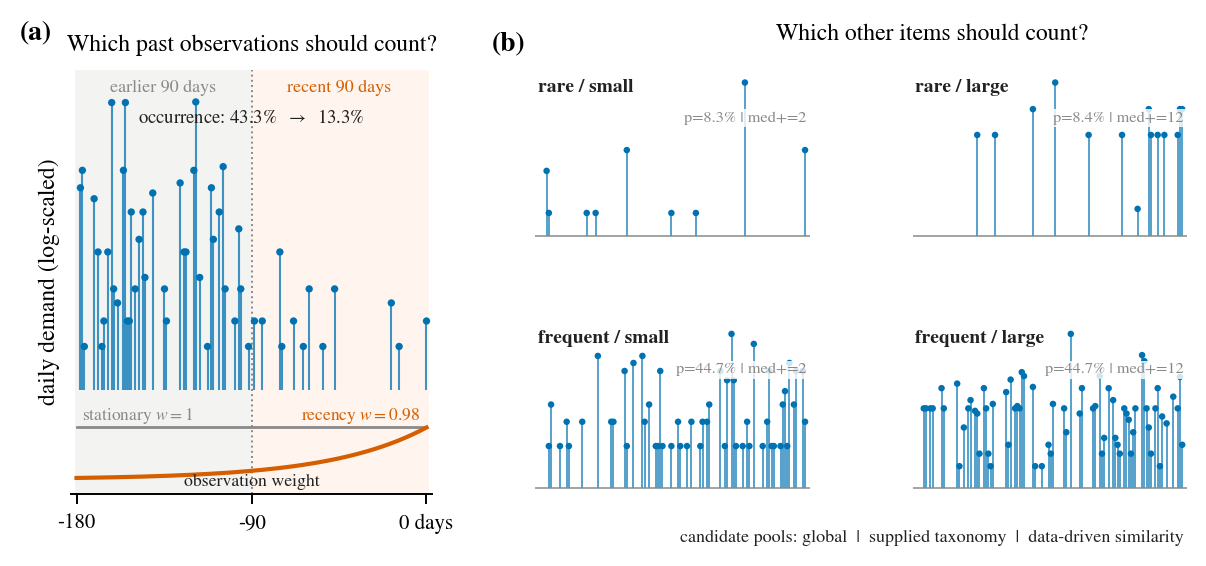
\includegraphics[width=0.98\textwidth]{fig01_problem.png}
\caption{The two coupled choices, in real intermittent demand.
\textbf{(a)} One item's daily history: occurrence falls from $43.3\%$ to
$13.3\%$ between the earlier and the recent ninety days, so a stationary
weighting ($w=1$) and a recency weighting ($w=0.98$) summarize the same
history differently---which past observations should count?
\textbf{(b)} Four items from the same panel, spanning rare and frequent
occurrence at small and large sizes: any pooled prior must decide which
of these heterogeneous neighbors an item should borrow strength
from---which other items should count? Candidate pools are a global
pool, a supplied taxonomy, and data-driven similarity.}
\label{fig:problem}
\end{figure*}

We operationalize this principle with
\REMIX{},\footnote{The name reflects the construction rather than an
acronym: recency-weighted evidence and cross-series pooling are
\emph{remixed} inside one empirical-Bayes family instead of being
specified as separate decisions.} a recency-weighted hierarchical
empirical-Bayes forecaster for intermittent demand. The model uses an
occurrence--size decomposition with Beta--Binomial occurrence and
log-normal size blocks, represented by per-item sufficient statistics. The
same exponential weights are applied to the statistics used for the item
posterior and for group-level hyperparameter estimation. A small candidate
family crosses discount factors with a global pool, the classical
ADI/CV$^2$ taxonomy, and BIC-selected mixture partitions; chronological
validation selects the pair before a full-window refit. For a fixed
candidate family, estimation is deterministic and linear in the number of
observations, with low-dimensional group optimization and mixture search.

The theory predicts an asymmetric empirical pattern. Forgetting should be
a first-order forecasting decision, whereas refining an already pooled
model can help only when the discounted data still resolve the proposed
groups. Because the resolution condition depends on quantities available
from the fitting window, it can be checked panel by panel before any
partition is fitted. The first half holds: all five panels select a
discount below one, and on the panel where both effects are measurable
forgetting is worth an order of magnitude more than refinement. The second
half fails in a more informative way than we expected. Refining the
pooling structure improves external accuracy on none of the five panels,
and the diagnostic shows this is not because the panels lack room. Three
of them retain substantial credibility leverage, and one---Online
Retail---sits at exactly the level where a supplied true partition earns
more than two percent in controlled study, while its learned partition
returns $-0.05\%$. What binds is therefore not the resolution limit but
learnability: the structure would pay if it were correct, and the mixture
objective does not find it. Separating those two explanations is what the
diagnostic is for, and it is the distinction between a resolution limit
and an absence of useful cross-series structure.

The resulting empirical position is deliberately narrow. Across the five
panels \REMIX{} attains the lowest mean scaled pinball loss on four, with
margins over the strongest comparator ranging from roughly one percent to
ten; an official Tweedie--Gaussian-process implementation is
better on Carparts and throughout that panel's far tail. Under strict
walk-forward updating the margin is $6.2\%$ over adaptive conformal
inference on Online Retail and $9.9\%$ over the strongest statistical
comparator on Carparts, and it is concentrated in the upper quantiles:
below the median, several methods on these panels coincide exactly with
the all-zero forecast. We report this structure rather than an aggregate
win because it is what the mechanism predicts, and because two widely used
evaluation conventions actively obscure it.

\paragraph{Contributions.}
\textbf{(1) Joint adaptation.} We introduce a scalable empirical-Bayes
model that applies one recency operator consistently to item- and
group-level sufficient statistics, then selects the discount jointly with
the pooling structure by leakage-free chronological validation. The
resulting predictive law is closed form, bit-reproducible, and costs
milliseconds per series on a CPU.
\textbf{(2) An estimable resolution condition.} We show that discounting
has two linked effects: it keeps prior leverage active but reduces the
information with which group heterogeneity can be estimated. A two-sided
credibility bound gives the collapse probability of the group variance
component, and its resolution corollary converts that bound into a
statistic computable from the fitting window. The statistic bounds how
much any partition could be worth on a given panel before one is fitted,
and separates a panel with no room from a panel whose room we fail to use.
Connections to TSB, drift tracking, classical credibility, and
finite-class selection are collected in the appendix.
\textbf{(3) Mechanism-focused evidence, including a negative result.}
Five real-data panels, two strict walk-forward evaluations, and a
known-partition simulation separate gains from forgetting, gains from
pooling refinement, and distortions caused by zero-favoring point metrics.
Comparators include the official TweedieGP implementation, adaptive
conformal inference, a published hierarchical state-space model, and a
zero-shot foundation model. Learned pooling improves external accuracy on
none of the five panels, and we show this is not attributable to a lack of
leverage: on the panel with the most room the learned partition still
loses. We also document two evaluation failures that the
intermittent-demand literature currently inherits---absolute-error metrics
reward the all-zero forecast, and static split-conformal wrappers
understate what conformal prediction can do here by about $20\%$.


% =========================================================================
% SECTION 2 — RELATED WORK  (replaces \section{Related Work} in full)
% =========================================================================
\section{Related Work}\label{sec:related}

\textbf{Intermittent-demand forecasting.} Croston's decomposition
\citep{croston1972}, its SBA correction \citep{syntetos2005accuracy}, and
TSB \citep{teunter2011} estimate occurrence and positive size locally;
TSB additionally lets the occurrence estimate decay under obsolescence.
ADIDA \citep{nikolopoulos2011} and IMAPA \citep{kourentzes2016} instead
reduce intermittency through temporal aggregation, while likelihood-based
alternatives include inventory count models \citep{snyder2012}, iETS
\citep{svetunkov2023iets}, Tweedie Gaussian processes \citep{damato2025},
and deep renewal processes \citep{turkmen2019}. Conformal wrappers turn
point forecasters into predictive intervals, and adaptive conformal
inference updates miscoverage levels under distribution shift
\citep{gibbs2021}; we evaluate both the static and the adaptive form,
because the difference between them is larger than most method
differences reported on these panels. These approaches provide important
forms of temporal adaptation, but do not jointly learn how
recency-weighted evidence should be shared across items. Hierarchical
models do share evidence: \citet{chapados2014} and \citet{seeger2016}
pool related count series at scale, and \citet{pitkin2024} develops a
hierarchical hurdle model for retail. Their pooling structure or temporal
evolution is generally specified in advance. \REMIX{} instead crosses
recency and pooling choices within one occurrence--size empirical-Bayes
model, and asks when that crossing can pay.

\textbf{Learning cross-series structure.} The continuum between local and
global forecasting is formalized by \citet{monteromanso2021}. More recent
work learns richer forms of cross-series specialization. For hierarchical
forecasting, \citet{cini2024} learns a graph-pooled aggregation hierarchy
aligned with the forecasting objective. Moirai-MoE \citep{liu2025moirai}
replaces human-defined frequency groups with token-level sparse-expert
routing in a time-series foundation model. These approaches motivate
data-adaptive structure, but address different objects: aggregation
coherence or latent expert specialization. Our groups are explicit
exchangeability pools for a shared prior. That restriction is what makes
their statistical resolution analyzable: the quantity governing whether a
pool can be estimated is the same credibility weight that governs whether
it can matter, so a single diagnostic covers both. It also permits a
direct comparison among global, fixed-rule demand-pattern, and learned
mixture pools under one predictive law.

\textbf{Discounting, credibility, and selection.} Exponential discounting
is classical in Bayesian dynamic models \citep{westharrison1997}, and
power priors down-weight historical likelihoods \citep{ibrahimchen2000}.
Likewise, $\lambda_i=n_i/(n_i+\phi_g)$ is the classical actuarial
credibility form \citep{buhlmann1967}; Proposition~\ref{prop:credibility}
is therefore a restatement, not a claimed contribution. The distinction in
\REMIX{} is that one recency operator updates both item statistics and the
empirical-Bayes statistics defining the shared prior, and its strength is
selected jointly with the pool. Proposition~\ref{prop:twosided} then
identifies the resulting two-sided resolution limit: forgetting preserves
prior leverage but can erase the information needed to distinguish fine
pools. Chronological validation selects among the finite candidate family.
Because zero-heavy point losses can favor degenerate forecasts, selection
uses pinball loss, a proper scoring rule \citep{gneiting2007}, with the
high quantiles relevant to inventory decisions \citep{kolassa2016}.

% =========================================================================
\section{\REMIX{}: Recency-Weighted Hierarchical EB}\label{sec:method}
% =========================================================================

\REMIX{} combines two candidate choices inside one occurrence--size
model: a recency discount $w$ determines which observations remain
informative, and a partition $g$ determines which items share an
empirical-Bayes prior. The key construction is that the \emph{same}
discounted sufficient statistics determine both the item posterior and
the group prior. We first define that representation, then the candidate
partitions and their leakage-safe joint selection.

\subsection{Occurrence--size model}\label{sec:base}

For item $i$, let $z_{i,t}=\ind{y_{i,t}>0}$ and define
$\ell_{i,t}=\log y_{i,t}$ when $z_{i,t}=1$. Conditional on membership
$g_i=g(i)$, the hurdle model is
\begin{equation}
\begin{aligned}
\pi_i &\sim \mathrm{Beta}(\alpha_{g_i},\beta_{g_i}), &
z_{i,t}\mid\pi_i &\sim \mathrm{Bern}(\pi_i),\\
\mu_i &\sim \mathcal{N}(\mu_{0,g_i},\tau^2_{g_i}),\\
\sigma_i^2 &\sim \mathrm{ScaleInv}\text{-}\chi^2
  (\nu,s^2_{0,g_i}),\\
\ell_{i,t}\mid z_{i,t}{=}1,\mu_i,\sigma_i^2
&\sim \mathcal{N}(\mu_i,\sigma_i^2).
\end{aligned}
\label{eq:model}
\end{equation}
Here $s^2_{0,g}$ is parameterized so that the prior mean of
$\sigma_i^2$ is the group estimate $\sigma_g^2$; $\nu$ is fixed rather
than selected. Group hyperparameters are estimated by empirical Bayes:
Beta--Binomial marginal likelihood for occurrence, and an
intercept-only random-effects fit plus conjugate variance shrinkage for
positive log-size. Appendix~\ref{app:implementation} gives the numerical
objectives and fallback rules.

Without forgetting, all inference depends on the four statistics
\[
S_i(1)=(n_i,c_i,u_i,v_i)
=\sum_{t=1}^{T_i}
  \bigl(1,z_{i,t},z_{i,t}\ell_{i,t},z_{i,t}\ell_{i,t}^2\bigr),
\]
where the last two terms are zero when $z_{i,t}=0$. The occurrence
posterior mean and the positive-size posterior location take parallel
credibility forms,
\begin{align}
\hat\pi_i
&=\lambda_i^{(o)}\bar p_i+(1-\lambda_i^{(o)})\mu_{\pi,g_i},
&\lambda_i^{(o)}&=\frac{n_i}{n_i+\phi_{g_i}},\nonumber\\
\hat\mu_i
&=\lambda_i^{(+)}\bar\ell_i+(1-\lambda_i^{(+)})\mu_{0,g_i},
&\lambda_i^{(+)}&=\frac{n_i^+}{n_i^++\kappa_{i,g_i}},
\label{eq:credibility-pair}
\end{align}
with $\phi_g=\alpha_g+\beta_g$ and
$\kappa_{i,g}=\hat\sigma_i^2/\tau_g^2$. Thus a partition matters only
through the prior target and strength supplied to its members.

Two variance ratios appear in what follows. Estimation uses the item-level
$\kappa_{i,g}=\hat\sigma_i^2/\tau_g^2$ in
\eqref{eq:credibility-pair}; the analysis in
Section~\ref{sec:resolution} works with the group-level surrogate
$\kappa_g=\sigma_g^2/\tau_g^2$, which replaces each item's process
variance by its group estimate. The two coincide when the group is
homogeneous in $\sigma_i^2$, and the surrogate is what the collapse event
of Proposition~\ref{prop:twosided} is stated in terms of.

The plug-in marginal predictive distribution is zero-inflated
log-normal:
\begin{equation}
\begin{aligned}
\Pr(Y_i=0\mid\mathcal D)&=1-\hat\pi_i,\\
\log Y_i\mid(Y_i>0,\mathcal D)
&\sim\mathcal N(\hat\mu_i,\hat\sigma_i^2+V_i),
\end{aligned}
\label{eq:predictive-law}
\end{equation}
where $V_i$ is posterior uncertainty in $\mu_i$. Its quantiles are
analytic. For point evaluation we retain the conditional plug-in mean
$\hat y_i=\hat\pi_i\exp(\hat\mu_i+\hat\sigma_i^2/2)$; it is distinct
from the mean of \eqref{eq:predictive-law}, which also integrates $V_i$.

\subsection{Shared recency weighting}\label{sec:discount}

For $w\in(0,1]$, replace $S_i(1)$ by
\begin{equation}
S_i(w)=\sum_{t=1}^{T_i}w^{T_i-t}
  \bigl(1,z_{i,t},z_{i,t}\ell_{i,t},z_{i,t}\ell_{i,t}^2\bigr).
\label{eq:discounted-stats}
\end{equation}
These fractional counts are valid weighted-likelihood statistics; the
log-Gamma form of the occurrence marginal and the Normal size objective
extend directly to them. Crucially, $S_i(w)$ is used twice:
\begin{equation}
\begin{aligned}
\widehat\eta_g(w)
&=\arg\max_{\eta_g}
  \sum_{i:g_i=g}\log m\{S_i(w)\mid\eta_g\},\\
q_i^{(w)}(\theta_i)
&=q_i\!\left(\theta_i\mid
  S_i(w),\widehat\eta_{g_i}(w)\right),
\end{aligned}
\label{eq:shared-recency}
\end{equation}
where $\eta_g$ collects the group hyperparameters and $q_i$ is the item
posterior. The group prior therefore adapts to recent cross-sectional
evidence rather than remaining a stationary prior applied to discounted
item data. Setting $w=1$ recovers the stationary estimator exactly.

For occurrence, \eqref{eq:credibility-pair} becomes
\begin{equation}
\begin{aligned}
\hat\pi_i(w)
&=\lambda_i(w)\bar p_i(w)
  +\{1-\lambda_i(w)\}\mu_{\pi,g_i}(w),\\
\lambda_i(w)
&=\frac{n_i(w)}{n_i(w)+\phi_{g_i}(w)}.
\end{aligned}
\label{eq:disc-post}
\end{equation}
The analogous positive-size update uses discounted positive mass
$n_i^+(w)$ and the group variance ratio $\kappa_{i,g}(w)$.

\subsection{Candidate pooling structures}\label{sec:mixture}

Let $\mathcal R$ contain three ways to construct $g(\cdot)$ from the
fitting data. Table~\ref{tab:pool-candidates} orders them from coarse to
fine: one prior for the panel, one prior per fixed demand-pattern class,
and one prior per learned component. The ladder is deliberate. The
question this paper asks is not which rung is best in general---that
depends on the panel---but whether the discounted data support moving up
it at all. Section~\ref{sec:resolution} gives the condition under which
they do, and Section~\ref{sec:main-results} reports what happens when they
do not.

\begin{table}[t]
\centering
\caption{Pooling candidates used by \REMIX{}, ordered coarse to fine.
Every data-dependent label is computed from the selector's fitting head,
never its validation tail.}
\label{tab:pool-candidates}
\small
\setlength{\tabcolsep}{3.5pt}
\begin{tabular}{lp{0.70\linewidth}}
\toprule
Candidate & Shared-prior groups\\
\midrule
Global & All items share one prior.\\
Taxonomy & Four ADI/CV$^2$ demand-pattern classes (smooth, intermittent,
erratic, lumpy) using the classical thresholds $1.32$ and $0.49$
\citep{syntetos2005categorization}.\\
Learned & Hard assignments from a mixture of occurrence--size prior
components; $K\in\{1,\ldots,6\}$ is selected by BIC.\\
\bottomrule
\end{tabular}
\end{table}

For the learned candidate, component $k$ carries
$\eta_k=(\alpha_k,\beta_k,\mu_{0,k},\tau_k^2,\sigma_k^2)$. Its item
marginal is the product of Beta--Binomial occurrence evidence and Normal
random-effects size evidence. EM has an analytic responsibility update;
its M-step maximizes responsibility-weighted EB objectives. A
deterministic quantile initialization makes repeated fits seed-free.
Mixture labels are built once from the fitting head and shared across the
discount grid, with $K\in\{1,\dots,6\}$ selected by BIC at that fit.
Re-learning the partition separately at every discount is a natural
variant---changing $w$ changes both the item evidence and the components
it can support---but we do not evaluate it here. The
selected responsibilities are converted to hard labels so all three
candidates share the same downstream forecaster.

\subsection{Leakage-safe joint selection}\label{sec:select}

Each training series is split chronologically into a fitting head
$\mathcal H_i$ (first $80\%$) and validation tail $\mathcal V_i$ (last
$20\%$). For every $(r,w)\in\mathcal R\times\mathcal W$, with
\[
\mathcal W=\{1,.999,.997,.995,.99,.98,.95,.90\},
\]
the partition builder for $r$ sees only $\mathcal H=\cup_i\mathcal H_i$.
The resulting labels, discounted EB prior, and item posteriors are all
fit on the same head. The candidate is scored by
\begin{equation}
\begin{aligned}
\widehat R(r,w)
&=\frac{1}{N_{\!V}}\sum_{i\in\mathcal I_V}
  \frac{1}{|\mathcal V_i||\mathcal Q|}\\[-0.25em]
&\quad\times
  \sum_{t\in\mathcal V_i}\sum_{q\in\mathcal Q}
  \frac{\rho_q(y_{i,t},\widehat Q_{i,t}^{(r,w)}(q))}{a_i},
\end{aligned}
\label{eq:selection-risk}
\end{equation}
where $\mathcal Q=\{.5,.75,.9\}$, $\rho_q$ is pinball loss, and $a_i$
is mean absolute demand on the fitting head (with a panel-level fallback
for an all-zero head); $N_V=|\mathcal I_V|$ is the number of scored
items. Times and quantiles are averaged within item
before items receive uniform weight. This matches the panel-level goal
and prevents long series or high-volume items from dominating selection.

The selected pair is
$(\hat r,\hat w)=\arg\min_{r,w}\widehat R(r,w)$. Its partition is then
\emph{relearned} on the complete training window at $\hat w$, and the EB
model is refit once before external evaluation. Thus the validation tail
chooses a construction rule and discount, not a permanent set of labels;
external targets are never used. There are 24 outer forecast candidates.

\paragraph{Resolution diagnostics.}
Fitting each candidate already produces everything the resolution
analysis of Section~\ref{sec:resolution} needs, so the selector records it
rather than recomputing it later. For every $(r,w)$ and every resulting
group $g$ we store, from the fitting head only, the median occurrence and
positive-size credibility weights $\lambda_i^{(o)}$ and $\lambda_i^{(+)}$,
the share of items with $\lambda_i^{(+)}<0.1$, the group sizes $m_g$, and
the resolution statistic
\[
\hat z_g=\frac{S_g^2-\bar s_g}{\sqrt{2/(m_g-1)}\,S_g^2},
\]
whose nonpositive values coincide with the collapse event
$\hat\tau_g^2=0$ of Proposition~\ref{prop:twosided}. These quantities cost
nothing beyond the fit that produced them, they are computed before any
external observation is seen, and they answer a question the validation
score cannot: not which candidate scores best on the tail, but whether the
discounted data contain enough information to estimate the candidate's
group structure at all. Section~\ref{sec:main-results} uses them to
separate the two. The full selection surface and the accompanying
diagnostics are released with every run
(\texttt{remix\_selection\_diagnostics.csv}).

Appendix~\ref{app:implementation} gives split edge cases and
pseudocode-level implementation details.

\subsection{Forecasts and computation}\label{sec:complexity}

Selection uses the analytic plug-in quantiles in
\eqref{eq:predictive-law}. The reported probabilistic forecasts also
average quantile estimates across $B=20$ cross-item bootstrap refits of
the group hyperparameters. We treat this explicitly as a quantile
ensemble; the average of component quantiles is not asserted to be the
quantile of a single posterior mixture.

For each $w$, one pass computes $S_i(w)$ in $O(\sum_iT_i)$ time. Each EB
fit requires only low-dimensional deterministic optimization per group;
mixture EM is $O(NK)$ per iteration. Prediction is $O(N)$ for points and
$O(NQ)$ for $Q$ quantiles.

Two properties of this cost profile matter for the comparisons that
follow. First, the whole pipeline is CPU-only and closed form apart from
the mixture search: fitting and predicting a panel costs on the order of
milliseconds per series, so the full 24-candidate joint selection
completes in minutes on a laptop-class machine and no GPU, tuning budget,
or convergence diagnostic is required. Second, estimation is exact rather
than approximate at every stage, so repeated end-to-end runs are
bit-identical in the released test suite. Neither property is an accuracy
claim; both are the terms on which the accuracy results in
Section~\ref{sec:experiments} should be read, since several of the
strongest comparators there cost two to three orders of magnitude more per
series and none is reproducible to the bit. Measured wall-clock figures
for every method are in Appendix~\ref{app:implementation}.

% =========================================================================
\section{Resolution under Forgetting}\label{sec:theory}
% =========================================================================

The shared operator in \eqref{eq:shared-recency} creates two opposing
effects. A bounded item history prevents the group prior from vanishing,
but the same bound limits the information used to estimate fine group
structure. This section formalizes that interaction. Supporting results
connecting the model to TSB, drift tracking, finite-class selection, and
classical credibility are collected in Appendix~\ref{app:supporting}.

\subsection{Persistent prior leverage}

Fix an item and suppress its subscripts. Because
$n(w)=\sum_{t=1}^{T}w^{T-t}\le(1-w)^{-1}$ for $w<1$, the occurrence
credibility weight cannot converge to one.

\begin{proposition}[Forgetting keeps pooling relevant]
\label{prop:active}
For every horizon $T$,
$\lambda(w)\le\{1+(1-w)\phi\}^{-1}<1$ when $w<1$, whereas
$\lambda(1)\to1$ as $T\to\infty$. Hence the pooled occurrence prior
retains positive weight indefinitely under forgetting.
\end{proposition}

The statement is about leverage, not benefit: it does not guarantee
that a particular prior is a good shrinkage target. It says that the
choice of target can continue to affect forecasts even for old series.

\subsection{Variance-component resolution}\label{sec:resolution}

The converse problem appears in the positive-size block. Let item $i$
in group $g$ have discounted positive mass $n_i^+$, sampling variance
$s_i=\sigma_g^2/n_i^+$ for its log-size mean, and credibility
$\lambda_i^{(+)}=n_i^+/(n_i^++\kappa_g)$ with
$\kappa_g=\sigma_g^2/\tau_g^2$. The group variance is estimated by the
truncated moment/REML form
$\hat\tau_g^2=\max(0,S_g^2-\bar s_g)$, where $S_g^2$ is the sample
variance of the $m_g$ item means and
$\bar s_g=m_g^{-1}\sum_{i\in g}s_i$.

\begin{proposition}[Two-sided effect of forgetting]
\label{prop:twosided}
\textbf{(i)} For $w<1$,
$\lambda_i^{(+)}\le\{1+(1-w)\kappa_g\}^{-1}<1$.
\textbf{(ii)} For independent item means with possibly unequal $s_i$,
\[
\E[S_g^2]=\tau_g^2+\bar s_g
\]
holds exactly. Under the Gaussian moment approximation,
\begin{equation}
\Pr(\hat\tau_g^2=0)\simeq
\Phi\!\left(-\sqrt{\frac{m_g-1}{2}}\,\rho_g\right),
\qquad
\rho_g=\frac{\tau_g^2}{\tau_g^2+\bar s_g}.
\label{eq:collapse-prob}
\end{equation}
Since $n_i^+\le(1-w)^{-1}$,
$\bar s_g\ge(1-w)\sigma_g^2$ and therefore
\[
\rho_g\le
\frac{\tau_g^2}{\tau_g^2+(1-w)\sigma_g^2}.
\]
On the collapse event the plug-in estimate has $\hat\tau_g^2=0$ and
$\lambda_i^{(+)}=0$: the item mean is replaced by its estimated group
mean.
\end{proposition}

The population ratio $\rho_g$ is not observed. For diagnostics we use
\[
\hat z_g=\frac{S_g^2-\bar s_g}
{\sqrt{2/(m_g-1)}\,S_g^2},
\]
whose nonpositive values coincide with the plug-in collapse event.

\begin{corollary}[Resolution condition]
\label{cor:resolution}
For this estimator and window, stable estimation of a group variance
requires, up to a fixed probability threshold,
\[
\rho_g\sqrt{m_g-1}\gtrsim1,
\qquad\text{or equivalently}\qquad
\tau_g^2\gtrsim
\frac{\bar s_g}{\sqrt{m_g-1}-1},
\]
with $\bar s_g\ge(1-w)\sigma_g^2$.
\end{corollary}

For similarity-based refinements, finer groups typically reduce both
$m_g$ and the within-group spread $\tau_g^2$, while stronger forgetting
raises the sampling-variance floor. All three changes move the estimator
toward collapse. This is an estimator- and window-specific resolution
condition, not an information-theoretic lower bound, and it does not say
which candidate wins below the threshold.

\begin{figure*}[!t]
\centering
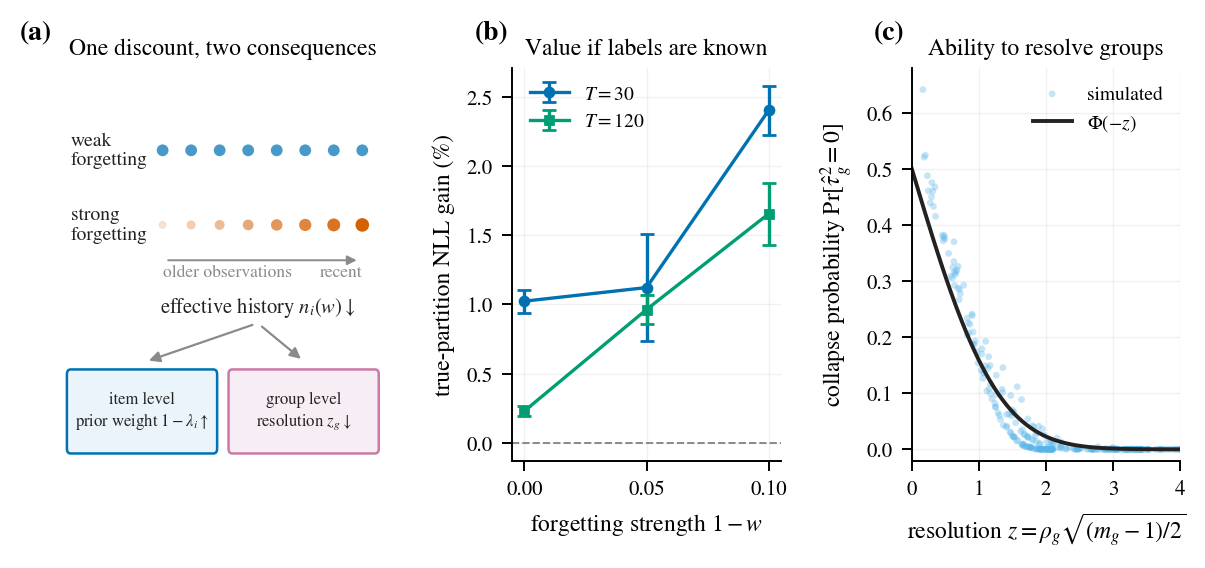
\includegraphics[width=0.98\textwidth]{fig01_mechanism.png}
\caption{\textbf{One discount creates two opposing effects.}
\textbf{(a)} The same recency operator reduces item effective history,
which increases prior leverage, and group effective information, which
reduces structural resolution. \textbf{(b)} In the controlled study, a
supplied true partition becomes more valuable as forgetting strengthens.
\textbf{(c)} When the partition must be estimated, the probability that
the group variance collapses rises as the resolution statistic falls;
the curve is the approximation in \eqref{eq:collapse-prob}.}
\label{fig:mechanism}
\end{figure*}

Figure~\ref{fig:mechanism} summarizes why pooling can become more
consequential at exactly the point where a fine partition becomes harder
to estimate. Section~\ref{sec:synthetic} tests both sides with known group
labels. Proofs and the accuracy limits of the approximation are given in
Appendix~\ref{app:proofs} and Section~\ref{sec:limitations}.
% Experiments are maintained separately so the main probabilistic narrative
% and the supporting appendix evidence can be edited as one coherent unit.
% =========================================================================
% REMIX v5 — sections/experiments.tex
% Composition: v4 full replacement (5.1–5.3) + v5 controlled study (5.4,
% moved before the leverage section) + v5 "When can pooling pay?" (5.5).
% All REMIX rows and margins use the audited configurations.
% =========================================================================

% =========================================================================
\section{Experiments}\label{sec:experiments}
% =========================================================================

\subsection{Experimental design}\label{sec:setup}

\textbf{Datasets.} We evaluate on two daily panels---\textbf{Online
Retail} \citep{chen2015} (3{,}649 series) and a seed-controlled
5{,}000-series \textbf{M5} sample \citep{makridakis2022}---and the
monthly intermittent suite of \citet{damato2025}: \textbf{Auto}
(3{,}000 series), \textbf{Carparts} (2{,}509), and \textbf{RAF}
(5{,}000). Together they contain more than 19{,}000 series and span
long daily histories and short, highly sparse monthly panels. Dataset
construction and holdout lengths are in Appendix~\ref{app:datasets}.
Both the probabilistic and the point M5 protocols use the first two
thirds of each series for initialization.

\textbf{Comparators.} The classical set comprises Croston, SBA, TSB,
ADIDA, and IMAPA; stronger statistical comparators are AutoARIMA,
AutoTheta, a per-series autoregressive Tweedie GLM, iETS, and the official
TweedieGP implementation on the three monthly panels. For probabilistic
evaluation we use native distributions where available and chronological
split-conformal wrappers (CP-$\ast$) for the point forecasters. The
Online Retail walk-forward study additionally includes adaptive conformal
inference (ACI) applied to ADIDA and TSB. A 25-candidate tuned-TSB control
receives the same internal chronological selection budget as \REMIX{}.
DeepState and Chronos-Bolt comparisons are confined to
Appendix~\ref{app:neural} because they use subset or proxy protocols.
Implementation details and complete settings are in
Appendix~\ref{app:implementation}.

\textbf{Protocols and metrics.} The primary fixed-origin experiment fits
once on the initialization window and scores the full evaluation span.
A strict walk-forward experiment then reveals and updates one block at a
time: seven-day blocks on Online Retail and one-month blocks on Carparts.
Classical and conformal methods refit each block except Online Retail
AutoARIMA, AutoTheta, and iETS, which refit every four blocks; \REMIX{}
updates discounted sufficient statistics each block. The primary metric is
scaled pinball loss (SPL; lower is better), averaged over
$q\in\{0.1,0.25,0.5,0.75,0.9\}$; we separately report q90 and the far tail
because inventory decisions are asymmetric. All quantiles are
zero-truncated and monotonized, and \REMIX{} is reported without post-hoc
calibration. Every model in Table~\ref{tab:prob} is scored by one
implementation from its stored quantile predictions, so no cell mixes
scoring versions. Fixed-origin, walk-forward, and subset foundation model
results are kept separate because they answer different questions. MAE and
RMSSE are secondary diagnostics rather than the headline criteria because
zero forecasts can minimize absolute error on intermittent panels. Full
point, interval, significance, and efficiency results are in
Appendix~\ref{app:extra}.

% =========================================================================
\subsection{Probabilistic forecasting across panels}
\label{sec:main-results}
% =========================================================================

\begin{table*}[t]
\centering
\caption{\textbf{Probabilistic forecasting is the primary comparison.}
Scaled pinball loss (SPL; lower is better) is reported as the mean over
$q\in\{0.1,0.25,0.5,0.75,0.9\}$ and at q90. Bold and underline mark the
best and second-best non-degenerate methods. M5 reports seed 42 for direct
comparability; three-seed robustness is summarized in the text. \REMIX{}
uses its raw predictive law, with no post-hoc calibration. TweedieGP is the
official implementation and is evaluated on the three monthly panels for
which the authors released it. The all-zero row is a metric diagnostic and
is excluded from ranking.}
\label{tab:prob}
\small
\setlength{\tabcolsep}{3.2pt}
\begin{tabular}{lcc@{\hspace{9pt}}cc@{\hspace{9pt}}cc@{\hspace{9pt}}cc@{\hspace{9pt}}cc}
\toprule
 & \multicolumn{2}{c}{Online Retail} & \multicolumn{2}{c}{M5} & \multicolumn{2}{c}{Auto} & \multicolumn{2}{c}{Carparts} & \multicolumn{2}{c}{RAF}\\
\cmidrule(lr){2-3}\cmidrule(lr){4-5}\cmidrule(lr){6-7}\cmidrule(lr){8-9}\cmidrule(lr){10-11}
Model & Mean & q90 & Mean & q90 & Mean & q90 & Mean & q90 & Mean & q90\\
\midrule
AutoARIMA & 1.0069 & 1.6297 & 1.7919 & 2.4148 & 0.3189 & 0.2659 & 0.4084 & 0.4897 & 0.4020 & 0.5910\\
AutoTheta & 1.0055 & \secondbest{1.6056} & 1.7954 & 2.3123 & 0.3403 & 0.2760 & 0.3925 & \secondbest{0.4697} & 0.4104 & 0.5956\\
CP-Croston & 1.5502 & 2.7686 & \secondbest{1.6902} & \best{2.1551} & 0.3260 & 0.3105 & 0.4012 & 0.5433 & 0.3322 & 0.4927\\
CP-SBA & 1.5492 & 2.8601 & 1.6939 & \secondbest{2.1736} & 0.3256 & 0.3153 & 0.3982 & 0.5418 & 0.3290 & 0.4920\\
CP-TSB & 1.1744 & 2.6746 & 1.8794 & 2.3148 & 0.3459 & 0.3150 & 0.3783 & 0.4842 & 0.3814 & 0.4986\\
CP-ADIDA & 1.1239 & 2.5409 & 1.7150 & 2.1949 & 0.3275 & 0.3082 & 0.3571 & 0.4982 & 0.3097 & 0.4905\\
CP-IMAPA & 1.1280 & 2.5506 & 1.7190 & 2.1904 & 0.3279 & 0.3084 & 0.3561 & 0.4908 & 0.3116 & 0.4907\\
Tweedie-GLM & 1.1477 & 1.7458 & 4.0693 & 5.2620 & 0.3221 & 0.2783 & 0.4776 & 0.6897 & 0.3121 & 0.5312\\
iETS & \secondbest{0.9846} & 1.7544 & 2.0282 & 2.9772 & 0.3448 & 0.3252 & 0.4561 & 0.5646 & 0.3494 & \secondbest{0.4900}\\
TweedieGP & --- & --- & --- & --- & \secondbest{0.2985} & \best{0.2598} & \best{0.3214} & \best{0.4600} & \secondbest{0.2763} & 0.5219\\
\midrule
Zero (diagnostic) & 0.9161 & 1.6490 & 1.9590 & 3.5262 & 0.5612 & 1.0102 & 0.3736 & 0.6725 & 0.2669 & 0.4805\\
\midrule
\REMIX{} (ours) & \best{0.8849} & \best{1.5268} & \best{1.6707} & 2.4758 & \best{0.2937} & \secondbest{0.2599} & \secondbest{0.3229} & 0.4817 & \best{0.2680} & \best{0.4856}\\
\bottomrule
\end{tabular}
\end{table*}

Table~\ref{tab:prob} sets the empirical position, and it is a narrow one.
\REMIX{} attains the lowest mean SPL on four of the five panels; the
official TweedieGP implementation wins Carparts ($0.3214$ versus
$0.3229$). The margins over the strongest comparator vary by an order of
magnitude across panels: $10.1\%$ on Online Retail, $3.0\%$ on RAF,
$1.6\%$ on Auto, and $1.2\%$ on M5. Across three independent
5{,}000-series M5 samples the selected configuration is identical---%
$(\text{mixture},\,w{=}0.95,\,K{=}6)$---and \REMIX{} has mean SPL
$1.7501\pm0.084$ against $1.7547\pm0.065$ for CP-Croston, its closest
comparator: ahead on two samples, behind by $1.0\%$ on the third, and
ahead on average by $0.3\%$, well within one standard deviation. We report
the spread rather than an aggregate win because it is the quantity
Section~\ref{sec:leverage} explains. The explanation is not that these
panels leave no room for a hierarchical construction to work; on three of
them the credibility weights say otherwise. It is that the room which
exists is not converted by a learned partition, which is why the
achievable margin is set by the shared predictive law rather than by the
pooling structure.

The degenerate row exposes what the central quantiles cannot see. On RAF,
the all-zero forecast is marginally better through q90 because the true
quantiles of most series are zero. At $q\in\{0.95,0.975,0.99\}$ it falls
behind every intensity-bearing method, and intensity-bearing models become
distinguishable from one another (Appendix~\ref{app:fartail}). TweedieGP
is strongest throughout the Carparts far tail and remains competitive on
RAF. The probabilistic claim is therefore not that one distribution wins
every quantile, but that \REMIX{} is the most consistent aggregate
performer across panels and remains informative in the region where a zero
forecast ceases to be useful.

Point forecasts tell a deliberately weaker story. \REMIX{} is best on six
of ten MAE/RMSSE cells and top two on seven, but the zero forecast has the
lowest MAE on three panels and classical methods lead several remaining
cells. We report the complete point table and horizon decomposition in
Appendix~\ref{app:point}: they establish competitiveness and rule out a
long-horizon averaging artifact, but do not support uniform point-forecast
superiority.

% =========================================================================
\subsection{Strict walk-forward forecasting}\label{sec:walkforward}
% =========================================================================

\begin{table*}[t]
\centering
\caption{\textbf{Strict probabilistic walk-forward evaluation.}
Online Retail uses seven-day blocks and Carparts uses monthly blocks.
Mean and q90 are scaled pinball losses; Cov.$^{+}$ is 80\% interval
coverage conditional on positive demand and AIW is average interval
width. Dashes denote an unevaluated panel. AutoTheta refits every four
Online Retail blocks; the classical wrappers, ACI, and all Carparts
baselines refit each block. \REMIX{} updates sufficient statistics each
block. Bold and underline rank non-degenerate methods by SPL.}
\label{tab:wfprob}
\footnotesize
\setlength{\tabcolsep}{4.0pt}
\begin{tabular}{lrrrrrrrr}
\toprule
 & \multicolumn{4}{c}{Online Retail} & \multicolumn{4}{c}{Carparts}\\
\cmidrule(lr){2-5}\cmidrule(lr){6-9}
Model & Mean & q90 & Cov.$^{+}$ & AIW & Mean & q90 & Cov.$^{+}$ & AIW\\
\midrule
AutoTheta & 1.0586 & \secondbest{1.4835} & 0.765 & 16.43 & 0.4056 & \secondbest{0.4743} & 0.678 & 1.80\\
CP-TSB & 1.3733 & 2.8422 & 0.468 & 5.71 & 0.3836 & 0.4758 & 0.551 & 1.27\\
CP-ADIDA & 1.1576 & 2.5143 & 0.473 & 5.47 & 0.3509 & 0.4880 & 0.593 & 1.28\\
CP-IMAPA & 1.1773 & 2.5224 & 0.471 & 5.47 & \secondbest{0.3492} & 0.4789 & 0.581 & 1.27\\
ACI-ADIDA & \secondbest{0.9108} & 1.6681 & 0.646 & 19.67 & --- & --- & --- & ---\\
Zero (diagnostic) & 0.9161 & 1.6490 & 0.000 & 0.00 & 0.3736 & 0.6725 & 0.000 & 0.00\\
\midrule
\REMIX{} & \best{0.8540} & \best{1.4002} & 0.621 & 10.31 & \best{0.3145} & \best{0.4578} & 0.669 & 1.41\\
\bottomrule
\end{tabular}
\end{table*}

Table~\ref{tab:wfprob} is the deployment-facing test. On Online Retail
\REMIX{} improves mean SPL by $6.2\%$ over ACI-ADIDA and q90 by $5.6\%$
over AutoTheta, the strongest q90 comparator. On Carparts it improves mean
SPL by $9.9\%$ over CP-IMAPA and wins all five quantiles.

Three features of this table deserve more attention than the margins.
First, \emph{the choice of conformal construction matters more here than
the choice of forecaster}: making the wrapper adaptive
\citep{gibbs2021} improves ADIDA's mean SPL from $1.1576$ to $0.9108$, a
$21\%$ gain that is more than three times the remaining gap to \REMIX{}.
Static split-conformal wrappers are the standard probabilistic baseline in
this literature; on this evidence they understate what conformal
prediction can do on intermittent panels, and comparisons drawn against
them---including earlier versions of our own---are correspondingly
generous. Second, \emph{coverage and sharpness separate}. ACI-ADIDA
attains higher positive-demand coverage ($0.646$ versus $0.621$) with
intervals almost twice as wide ($19.67$ versus $10.31$); neither method
dominates, and the SPL ordering reflects sharpness rather than
calibration. Third, \emph{the central quantiles carry little information
on the sparse panel}: on Carparts the q10 and q25 entries of \REMIX{}
equal the all-zero forecast exactly and q50 sits marginally below it, so
essentially the entire mean-SPL difference is generated above the median.
We return to this in Appendix~\ref{app:fartail}, where the far-tail
levels are the only ones that separate intensity-bearing models on the
sparsest panels.

The configuration is selected once at the origin and then updated online;
repeated online re-selection is outside the present experiment.

% =========================================================================
\subsection{Controlled test of the resolution mechanism}
\label{sec:synthetic}
% =========================================================================

Real data never reveal the true pooling partition, so on their own they
cannot distinguish a partition that is not worth having from one we failed
to find. Both appear as a small number. We therefore construct panels
where the partition is correct by definition, and use them as a reference
against which the learned partitions of Section~\ref{sec:leverage} are
measured: what a good partition is worth at a given level of credibility
leverage, rather than what our estimator obtains there.

We simulate from the hierarchical hurdle model of \eqref{eq:model} with
group centers arranged symmetrically around a fixed grand mean, so that
increasing separation does not change the panel scale. Each cell compares
a single pool against the known true partition under the same predictive
representation, with nine paired replicates, and sweeps the two quantities
that Section~\ref{sec:resolution} identifies as controlling credibility:
the discount $w$ and the series length $T$. The resulting grid spans the
leverage range the real panels occupy, from the near-fully-shrunk regime
of Carparts to the item-dominated regime of Auto and RAF.

\begin{table}[t]
\centering
\caption{Advantage of the \emph{true} partition over a single pool on
simulated panels (mean percentage improvement over nine paired replicates;
standard error in parentheses). Positive favors the partition. $T$ is
series length.}
\label{tab:sanity}
\small
\setlength{\tabcolsep}{3.5pt}
\begin{tabular}{llrrrr}
\toprule
$T$ & $w$ & NLL & log-size MSE & pinball & MAE\\
\midrule
$30$ & $0.90$ & $2.40\;(0.18)$ & $17.15\;(2.39)$ & $2.25\;(0.61)$ & $-1.72\;(0.73)$\\
$30$ & $0.95$ & $1.12\;(0.39)$ & $9.00\;(2.45)$ & $-0.44\;(0.58)$ & $-0.17\;(0.51)$\\
$30$ & $1.00$ & $1.02\;(0.08)$ & $8.37\;(1.53)$ & $-0.69\;(0.32)$ & $-1.95\;(0.59)$\\
$120$ & $0.90$ & $1.65\;(0.22)$ & $18.36\;(1.56)$ & $1.57\;(0.64)$ & $-3.34\;(1.37)$\\
$120$ & $0.95$ & $0.96\;(0.11)$ & $3.65\;(0.77)$ & $0.23\;(0.28)$ & $-1.32\;(0.73)$\\
$120$ & $1.00$ & $0.23\;(0.04)$ & $1.13\;(0.31)$ & $-0.32\;(0.13)$ & $-0.80\;(0.11)$\\
\bottomrule
\end{tabular}
\end{table}

Table~\ref{tab:sanity} gives the result. The true partition improves NLL
and log-size MSE in every cell, and pinball loss whenever forgetting is
strong; in a separate length sweep its pinball advantage decays from
$1.53\%$ at $T=12$ to $0.01\%$ at $T=400$. Both patterns follow the
credibility mechanism directly. Discounting or short histories reduce an
item's own weight $\lambda^{(+)}_i$ and open room for a prior to act;
long undiscounted histories drive $\lambda^{(+)}_i\to1$ and make every
partition irrelevant. Stronger forgetting simultaneously makes group
variance components harder to estimate, as
Proposition~\ref{prop:twosided} predicts, which is why the gains in the
$w=0.90$ rows are bought against a noisier $\hat\tau_g^2$ and do not
continue to grow without limit.

MAE moves the other way in all six cells. A known-correct partition, on
data generated from the model it describes, is reported as harmful by the
metric most commonly used in this literature. We take this as the cleanest
available statement of why Section~\ref{sec:main-results} treats
absolute-error criteria as diagnostics rather than as the headline.

\paragraph{What these panels are for.}
Plotted against median $\lambda^{(+)}$, the cells of
Table~\ref{tab:sanity} and the length sweep trace the grey curves of
Figure~\ref{fig:refinement-leverage}: the return to \emph{correct}
structure as a function of leverage. Because the partition is supplied
rather than estimated, that return is an upper envelope---no procedure
that must also learn the grouping can exceed it, and any procedure that
falls below it is losing something to estimation rather than to a lack of
structure. This is the comparison Section~\ref{sec:leverage} draws, and it
is the reason the controlled study is necessary rather than decorative:
the real panels supply the leverage coordinates, and only a known-partition
experiment can supply the ordinate they should be judged against.

Two boundaries apply. The experiment isolates the value of correct
structure and says nothing about whether the mixture recovers it---indeed
Section~\ref{sec:leverage} shows it does not, and the gap between the two
is precisely what the comparison measures. And it simulates from the model
that \REMIX{} fits, so the mechanism is tested under correct specification
only; a misspecified size law would shift the envelope, though it is hard
to see how it would raise it. Full diagnostics, including the growth of
$\mathrm{RMSE}(\hat\tau_g^2)$ as $w$ falls, are in
Appendix~\ref{app:simulation-details}.

% =========================================================================
\subsection{When can pooling pay?}\label{sec:leverage}
% =========================================================================

The results so far are consistent and small. This section asks whether
their size is a property of the data or of our estimator, and shows that
the two can be told apart with quantities the selector already computes on
the fitting head (Section~\ref{sec:select}).

\paragraph{What gets selected, and how weakly.}
All five panels select $w<1$: Carparts $0.90$, Online Retail and M5
$0.95$, Auto $0.99$, and RAF $0.997$. Across three independent
5{,}000-series M5 samples the selected configuration is identical in
structure, discount, and mixture order---$(\text{mixture},\,w{=}0.95,\,
K{=}6)$ in every case.

The pooling axis behaves differently, and the honest summary is that it
barely resolves. On three panels the spread between the best and worst
pooling structure at the selected discount is under a tenth of a percent
of validation SPL: $0.05\%$ on Online Retail, $0.08\%$ on Carparts,
$0.02\%$ on RAF. Only two panels separate at all---M5, where the learned
mixture beats the global pool by $0.58\%$, and Auto, where the global pool
beats every refinement by $0.31\%$. Announcing a winner on the other three
would report selector noise. What the selector reliably does is choose a
discount and avoid poor structural corners; it does not discover demand
taxonomies, and we do not claim it does.

\begin{table}[t]
\centering
\caption{\textbf{Credibility leverage under a single pool.} Median
credibility weight per panel at no forgetting and at the selected
discount, for both blocks of the hurdle model:
$\lambda^{(o)}_i=n_i/(n_i+\phi_g)$ for occurrence and
$\lambda^{(+)}_i=n_i^{+}/(n_i^{+}+\kappa_g)$ for positive size, the
latter being the quantity bounded by Proposition~\ref{prop:twosided}.
A weight near one means the item's own history dominates its posterior,
bounding how far any shared prior can move it. ``$<0.1$'' is the share of
items whose size-block weight falls below $0.1$. The final column is the
external MAE change of a separately selected learned partition relative to
the single pool; negative favors the single pool.}
\label{tab:leverage}
\small
\setlength{\tabcolsep}{3.0pt}
\begin{tabular}{lccccccc}
\toprule
 & & \multicolumn{3}{c}{$\lambda^{(+)}$ (size)} & \multicolumn{2}{c}{$\lambda^{(o)}$ (occ.)} & learned\\
\cmidrule(lr){3-5}\cmidrule(lr){6-7}
Panel & $w^{*}$ & $w{=}1$ & $w^{*}$ & $<0.1$ & $w{=}1$ & $w^{*}$ & vs.\ pool\\
\midrule
Carparts & $0.90$ & 0.802 & \textbf{0.224} & 22.5\% & 0.882 & 0.628 & $-1.2\%$\\
Online Retail & $0.95$ & 0.897 & \textbf{0.553} & 14.6\% & 0.969 & 0.895 & $-2.9\%$\\
M5 & $0.95$ & 0.996 & 0.841 & 12.9\% & 0.998 & 0.931 & $-2.3\%$\\
Auto & $0.99$ & 0.944 & 0.940 & 0.0\% & 0.525 & \textbf{0.422} & $-3.6\%$\\
RAF & $0.997$ & 0.926 & 0.917 & 0.0\% & 0.085 & \textbf{0.106} & $-31.5\%$\\
\bottomrule
\end{tabular}
\end{table}

\paragraph{Leverage is an upper bound, not a prediction.}
Table~\ref{tab:leverage} reports the diagnostic. Read as
Corollary~\ref{cor:resolution} intends, it does not say which partition
wins; it says how much any partition could win by. Two panels have almost
no room on the size block: Auto and RAF retain median
$\lambda^{(+)}\approx0.92$--$0.94$ even at their selected discounts, with
no item below $0.1$, so their sub-percent pooling differences are
explained before any partition is fitted. The remaining three do have
room. Carparts is extreme---median $0.224$, with $22.5\%$ of items
essentially fully shrunk---and Online Retail, at $0.553$ under the
selected discount, sits squarely in the regime where
Section~\ref{sec:synthetic} shows a supplied true partition earning more
than two percent.

\begin{figure}[t]
\centering
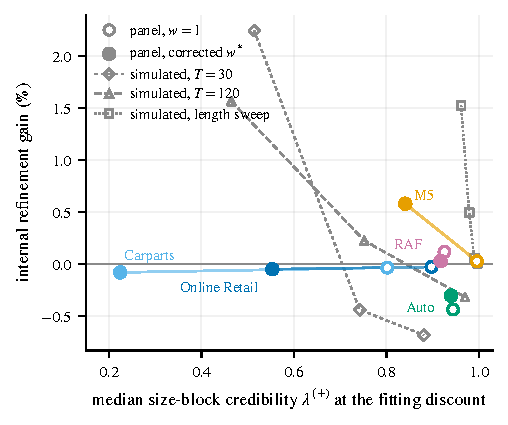
\includegraphics[width=\columnwidth]{figs/fig10a_refinement_leverage_size.pdf}\\[0.5em]
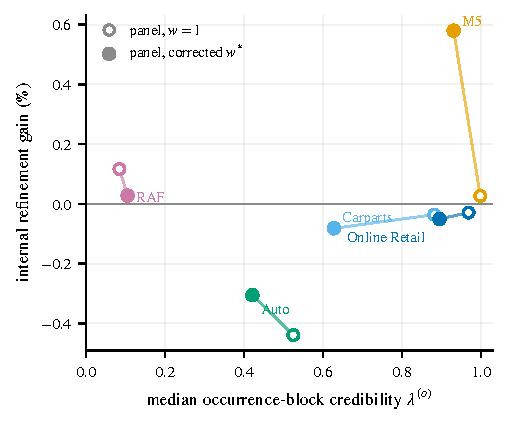
\includegraphics[width=\columnwidth]{figs/fig10b_refinement_leverage_occ.pdf}
\caption{\textbf{The simulated curves are an upper envelope that the real
panels do not reach.} Internal refinement gain (best refined structure
versus the global pool, validation SPL) against median credibility weight,
on the size block (top) and the occurrence block (bottom). Open markers
are $w{=}1$, filled markers the selected discount, and the connecting
segment is the movement forgetting induces. Grey curves are the controlled
panels of Section~\ref{sec:synthetic}, where the partition supplied is
correct by construction. Every real panel lies far below the envelope at
its own leverage---most visibly Online Retail, which the selected
discount moves into the high-return region of the size block while its
learned structure returns $-0.05\%$.}
\label{fig:refinement-leverage}
\end{figure}

\paragraph{What binds is learnability, not leverage.}
Figure~\ref{fig:refinement-leverage} places the real panels and the
controlled panels on the same axes, and the gap between them is the
section's main result. Where the partition is correct by construction, the
gain rises as leverage rises, reaching $+2.2\%$ near
$\lambda^{(+)}\approx0.5$. Where the partition must be learned, the gain
is between $-0.31\%$ and $+0.03\%$ on four panels and $+0.58\%$ on the
fifth, regardless of leverage. Online Retail is the decisive case: the
selected discount moves it to $\lambda^{(+)}=0.553$, inside the region
where the controlled study says a good partition is worth more than two
percent, and the mixture returns $-0.05\%$. The occurrence block behaves
the same way (Figure~\ref{fig:refinement-leverage}, bottom): RAF and Auto
occupy the low-$\lambda^{(o)}$ end, where the shared prior supplies most
of $\hat\pi_i$, and their refinement gains are still zero or negative.

This separates two explanations that aggregate results cannot. It is not
that these panels lack exploitable cross-series structure---the
credibility weights say the structure would be worth something if it were
correct. It is that the mixture objective does not recover a partition
worth shrinking toward. The binding constraint is learnability, and
Corollary~\ref{cor:resolution} bounds the prize rather than the shortfall.

\paragraph{High leverage is an amplifier with no sign attached.}
The clearest illustration is RAF, which combines the highest size-block
leverage in the panel set ($\lambda^{(+)}=0.917$) with the lowest
occurrence leverage ($\lambda^{(o)}=0.106$), and loses $31.5\%$ of
external MAE to a learned partition. The two facts are one fact. The point
forecast is $\hat y_i=\hat\pi_i\exp(\hat\mu_i+\hat\sigma_i^2/2)$; when
$89\%$ of $\hat\pi_i$ comes from the group prior, replacing the group is
close to replacing the forecast. This is the empirical content of the
caveat attached to Proposition~\ref{prop:active}: persistent prior leverage
guarantees that the choice of target keeps mattering, not that a
particular target is good. Read together with the previous paragraph, low
leverage caps the upside and high leverage uncaps the downside, and
neither makes a learned partition worth using here.

\paragraph{Forgetting is an order of magnitude larger.}
Computed within a single selection surface under one definition---the
M5 surface at its selected discount---refining the pooling
structure is worth $+0.58\%$ of validation SPL, while discounting at the
same structure is worth $8.95\%$ for the global pool and $9.46\%$ for the
mixture. The asymmetry that motivates the paper survives at an order of
magnitude, and it survives on the one panel where refinement is
measurable at all.

\begin{table}[t]
\centering
\caption{Online Retail distributional ablation. Each row is an
independent hierarchical run; ``auto'' denotes its own internal discount
selection. The raw predictive law is used and lower is better. Full
point metrics are in Appendix Table~\ref{tab:ablation-full}.}
\label{tab:ablation}
\small
\begin{tabular*}{\columnwidth}{@{\extracolsep{\fill}}llrrr@{}}
\toprule
Pooling & Forget & SPL & SPL$_{90}$ & AIW\\
\midrule
global & off & 0.8899 & 1.5306 & 10.51\\
taxonomy & off & 0.8897 & 1.5299 & 10.56\\
learned & off & 0.8905 & 1.5336 & 10.79\\
global & auto ($.95$) & \secondbest{0.8849} & \secondbest{1.5268} & \best{9.25}\\
taxonomy & auto ($.95$) & \best{0.8846} & \best{1.5254} & 9.43\\
learned & auto ($.95$) & 0.8869 & 1.5343 & 10.69\\
\bottomrule
\end{tabular*}
\end{table}

\paragraph{What the ablation confirms.}
Table~\ref{tab:ablation} is the external counterpart on Online Retail: the
three pooling candidates differ by less than $0.1\%$ in mean SPL without
forgetting and by less than $0.3\%$ at the selected discount, matching the
internal picture. Discounting shows up
elsewhere, narrowing the global and taxonomy $80\%$ intervals by
$11$--$12\%$ while improving mean SPL by about half a percent; the full
ablation
(Appendix Table~\ref{tab:ablation-full}) shows it improves external MAE by
$3.5$--$4.0\%$ and slightly worsens RMSE. The cross-panel result in
Table~\ref{tab:prob} should therefore be attributed to the shared
hurdle-EB predictive law and to the temporal half of the selection, not to
a learned-partition gain. That is not a concession made after the fact:
the leverage diagnostic states the ceiling in advance, and
Figure~\ref{fig:refinement-leverage}\ shows we do not reach it.


\section{Limitations}\label{sec:limitations}
% =========================================================================

\textbf{(1) The size law.} The log-normal positive-size block keeps
item-posterior updates analytic, but its tail is conservative on panels
with heavy-tailed spikes. Official TweedieGP is better on Carparts and
throughout that panel's far tail, and conformal wrappers are better at q90
on M5. A Gamma or Tweedie size block inside the same hierarchy is the
natural next instantiation, and Table~\ref{tab:prob} indicates where it
would pay.

\textbf{(2) Saturation and calibration.} Raw intervals over-cover on the
sparsest panels (Table~\ref{tab:coverage}), and on RAF the standard
quantile levels saturate: the all-zero forecast attains a marginally lower
mean SPL than every method. The far-tail levels ($q\ge0.95$) resolve this
(Appendix~\ref{app:fartail}), but CRPS and a cost-based criterion remain
unrun.

\textbf{(3) Assumptions behind the resolution condition.}
Corollary~\ref{cor:resolution} uses a Gaussian working model for the item
means and a $\chi^2$ approximation for $S_g^2$, accurate except for small
groups combining strongly unequal counts with strongly unequal sampling
variances, where it understates the collapse probability by up to $0.21$.
It is an estimator-specific estimability statement, not an
information-theoretic impossibility result. Section~\ref{sec:leverage}
shows the practical consequence of that distinction: the bound is an upper
envelope, and on these panels it is not the binding constraint.

\textbf{(4) The learnability gap is demonstrated, not closed.} Our
strongest negative result---leverage exists and the learned partition does
not exploit it---identifies a target rather than hitting it. Two
extensions are directly implicated and neither is bounded by
Corollary~\ref{cor:resolution} in the same way. A soft-responsibility
predictive mixture adds one matrix multiply and changes the \emph{shape}
of the predictive distribution rather than only the prior it shrinks
toward, which is where Table~\ref{tab:prob} locates our remaining
weakness. A partition objective that maximizes between-group separation
subject to keeping $\rho_g\sqrt{m_g}$ above threshold would target
learnability directly rather than likelihood. We report the gap because we
can measure it, not because we have closed it.

\textbf{(5) Baseline and inference scope.} We do not run external
hierarchical Bayesian implementations
\citep{chapados2014,seeger2016,pitkin2024}; claims about them are limited
to their published computational profiles.
Appendix~\ref{app:mcmc} closes the inference-method half of this gap---a
four-chain full-posterior Gibbs sampler matches plug-in EB within $0.1\%$
on SPL---so the EB approximation is not the distributional-accuracy
bottleneck, but the model-class half remains open. Our adaptive conformal
comparison is one ACI design, not an exhaustive study of weighted or
model-specific conformal methods; given how much it changed the baseline
(Section~\ref{sec:walkforward}), the remaining designs deserve more
attention than they have received in this literature. DeepState,
Chronos-Bolt, and Deep Renewal Process comparisons use subset or proxy
protocols and are reported only in Appendix~\ref{app:neural}.

\textbf{(6) Criterion and deployment alignment.} Selection uses a single
pinball-based score; the selector tracks whichever criterion it is given
(Section~\ref{sec:criterion}), but a cross-objective study including an
inventory cost criterion is future work. The discount is selected under
the fixed-origin protocol and reused in walk-forward: we keep the
initialization discount and the online block update distinct and do not
compound them, and we do not evaluate re-selection at every block.
Appendix~\ref{app:extra} records the remaining protocol details, including
the reduced refit cadence for AutoARIMA, AutoTheta, and iETS on Online
Retail.

% =========================================================================
\section{Conclusion}\label{sec:conclusion}
% =========================================================================

Intermittent-demand forecasting requires two structural choices: how
strongly to discount the past, and how to pool evidence across items.
\REMIX{} makes both by chronological validation inside a scalable
sufficient-statistic empirical-Bayes family, applying one recency operator
to item- and group-level statistics alike. Across five public panels it
attains the lowest mean scaled pinball loss on four, with an official
Tweedie--Gaussian-process specialist ahead on Carparts by half a percent,
and it leads under strict walk-forward updating on both a long daily and a
short monthly panel. These are distributional results obtained from a
closed-form, CPU-only, bit-reproducible predictive law; point forecasts
are competitive but not uniformly best.

The two choices turn out to be asymmetric, and the asymmetry is the
paper's finding. Discounting is a first-order decision: all five panels
select it, and on the one panel where both effects are measurable it is
worth an order of magnitude more than refining the pooling structure.
Refinement, by contrast, improves external accuracy on none of the five
panels and exceeds selector noise on only one.

Why it fails is the more useful result. Forgetting has two opposing
effects on pooling---it keeps a shared prior's leverage alive while
eroding the information that would resolve fine group structure---and the
resulting credibility weight bounds how much any partition could be worth.
That bound is real but not binding. Three panels retain substantial room,
and one of them, Online Retail, sits at the leverage where a supplied true
partition earns more than two percent in controlled study; its learned
partition returns $-0.05\%$. The constraint on cross-series pooling in
these data is therefore learnability rather than leverage: the structure
would pay if it were correct, and current mixture objectives do not find
it. Separating those two explanations required the diagnostic, and the
diagnostic costs nothing beyond the fit that produces it.

Two evaluation conventions actively obscure this picture, and both are
inherited rather than incidental. Absolute-error metrics reward the
all-zero forecast on three of five panels and reverse the ranking of a
known-correct partition in simulation; they should not be the sole basis
for comparing intermittent-demand forecasters. Static split-conformal
wrappers, the field's standard probabilistic baseline, understate what
conformal prediction achieves here by roughly twenty percent relative to
an adaptive construction---a margin several times larger than most method
differences reported on these panels, including our own.

The practical value of \REMIX{} is accordingly not a claim of universal
accuracy but a cheap, deterministic predictive distribution together with
an ex ante account of when temporal adaptation and finer pooling can
matter. The most direct next steps follow from the gap the diagnostic
exposes: partition objectives that optimize resolvable separation rather
than marginal likelihood, predictive mixtures that alter distributional
shape rather than only the shrinkage target, and decision-aware sequential
selection.

% =========================================================================
\section*{Reproducibility Statement}
All five datasets are public (UCI 352; Kaggle M5-Accuracy; the gluon-ts
\texttt{intermittent-datasets} branch for Auto and RAF; Zenodo record
4656022 for Carparts). Conversion and preprocessing scripts are included
in the released code. The full pipeline uses deterministic low-dimensional
EB optimization and seed-free quantile-based EM initialization, so no seed
policy is required for the forecaster itself. The stochastic elements are
the seed-controlled M5 subsample and the $B{=}20$ bootstrap; M5 results
are reported for seed~42 in the main tables and audited across three
independently drawn samples, which select the same configuration in every
case. An automated test asserts that two end-to-end runs are
bit-identical. Every table maps to one experiment directory via a manifest
file, and each run writes its selection diagnostics---chosen partition,
discount, BIC curves, and credibility leverage---alongside its metrics. Hardware and
timing methodology are specified in Appendix~\ref{app:implementation}.
The complete experiment suite runs on one CPU workstation in under a
day, dominated by the statistical baselines rather than \REMIX{}. An
anonymized code repository will accompany the submission.

\begin{thebibliography}{99}

\bibitem[B\"uhlmann(1967)]{buhlmann1967}
H.~B\"uhlmann.
\newblock Experience rating and credibility.
\newblock \emph{ASTIN Bulletin}, 4(3):199--207, 1967.

\bibitem[Chapados(2014)]{chapados2014}
N.~Chapados.
\newblock Effective Bayesian modeling of groups of related count time series.
\newblock In \emph{ICML}, 2014.

\bibitem[Chen(2015)]{chen2015}
D.~Chen.
\newblock Online Retail dataset, UCI Machine Learning Repository, 2015.

\bibitem[Cini et~al.(2024)]{cini2024}
A.~Cini, D.~Mandic, and C.~Alippi.
\newblock Graph-based time series clustering for end-to-end hierarchical
  forecasting.
\newblock In \emph{ICML}, volume 235 of PMLR, pages 8985--8999, 2024.

\bibitem[Croston(1972)]{croston1972}
J.~D. Croston.
\newblock Forecasting and stock control for intermittent demands.
\newblock \emph{Operational Research Quarterly}, 23(3):289--303, 1972.

\bibitem[Damato et~al.(2025)]{damato2025}
S.~Damato, D.~Azzimonti, and G.~Corani.
\newblock Forecasting intermittent time series with Gaussian processes and
  Tweedie likelihood.
\newblock \emph{International Journal of Forecasting}, 2025.

\bibitem[Gibbs and Cand\`es(2021)]{gibbs2021}
I.~Gibbs and E.~Cand\`es.
\newblock Adaptive conformal inference under distribution shift.
\newblock In \emph{NeurIPS}, 2021.

\bibitem[Gneiting and Raftery(2007)]{gneiting2007}
T.~Gneiting and A.~E. Raftery.
\newblock Strictly proper scoring rules, prediction, and estimation.
\newblock \emph{JASA}, 102(477):359--378, 2007.

\bibitem[Ibrahim and Chen(2000)]{ibrahimchen2000}
J.~G. Ibrahim and M.-H. Chen.
\newblock Power prior distributions for regression models.
\newblock \emph{Statistical Science}, 15(1):46--60, 2000.

\bibitem[Keribin(2000)]{keribin2000}
C.~Keribin.
\newblock Consistent estimation of the order of mixture models.
\newblock \emph{Sankhy\=a A}, 62(1):49--66, 2000.

\bibitem[Kolassa(2016)]{kolassa2016}
S.~Kolassa.
\newblock Evaluating predictive count data distributions in retail sales
  forecasting.
\newblock \emph{International Journal of Forecasting}, 32(3):788--803, 2016.

\bibitem[Kourentzes and Petropoulos(2016)]{kourentzes2016}
N.~Kourentzes and F.~Petropoulos.
\newblock Forecasting with multivariate temporal aggregation.
\newblock \emph{Int.\ J.\ Production Economics}, 181:145--153, 2016.

\bibitem[Lei et~al.(2018)]{lei2018}
J.~Lei, M.~G'Sell, A.~Rinaldo, R.~J. Tibshirani, and L.~Wasserman.
\newblock Distribution-free predictive inference for regression.
\newblock \emph{JASA}, 113(523):1094--1111, 2018.

\bibitem[Liu et~al.(2025)]{liu2025moirai}
X.~Liu, J.~Liu, G.~Woo, T.~Aksu, Y.~Liang, R.~Zimmermann, C.~Liu,
  J.~Li, S.~Savarese, C.~Xiong, and D.~Sahoo.
\newblock Moirai-MoE: Empowering time series foundation models with sparse
  mixture of experts.
\newblock In \emph{ICML}, volume 267 of PMLR, pages 38940--38962, 2025.

\bibitem[Makridakis et~al.(2022)]{makridakis2022}
S.~Makridakis, E.~Spiliotis, and V.~Assimakopoulos.
\newblock M5 accuracy competition: Results, findings, and conclusions.
\newblock \emph{International Journal of Forecasting}, 38(4):1346--1364, 2022.

\bibitem[Montero-Manso and Hyndman(2021)]{monteromanso2021}
P.~Montero-Manso and R.~J. Hyndman.
\newblock Principles and algorithms for forecasting groups of time
  series: Locality and globality.
\newblock \emph{International Journal of Forecasting}, 37(4):1632--1653,
  2021.

\bibitem[Nikolopoulos et~al.(2011)]{nikolopoulos2011}
K.~Nikolopoulos, A.~A. Syntetos, J.~E. Boylan, F.~Petropoulos, and
  V.~Assimakopoulos.
\newblock An aggregate--disaggregate intermittent demand approach (ADIDA).
\newblock \emph{JORS}, 62(3):544--554, 2011.

\bibitem[Pitkin et~al.(2024)]{pitkin2024}
J.~Pitkin, I.~Manolopoulou, and G.~Ross.
\newblock Bayesian hierarchical modelling of sparse count processes in
  retail analytics.
\newblock \emph{Annals of Applied Statistics}, 18(2):946--965, 2024.

\bibitem[Salinas et~al.(2020)]{salinas2020}
D.~Salinas, V.~Flunkert, J.~Gasthaus, and T.~Januschowski.
\newblock DeepAR: Probabilistic forecasting with autoregressive recurrent
  networks.
\newblock \emph{International Journal of Forecasting}, 36(3):1181--1191, 2020.

\bibitem[Seeger et~al.(2016)]{seeger2016}
M.~Seeger, D.~Salinas, and V.~Flunkert.
\newblock Bayesian intermittent demand forecasting for large inventories.
\newblock In \emph{NeurIPS}, 2016.

\bibitem[Snyder et~al.(2012)]{snyder2012}
R.~D. Snyder, J.~K. Ord, and A.~Beaumont.
\newblock Forecasting the intermittent demand for slow-moving
  inventories: A modelling approach.
\newblock \emph{International Journal of Forecasting}, 28(2):485--496,
  2012.

\bibitem[Svetunkov and Boylan(2023)]{svetunkov2023iets}
I.~Svetunkov and J.~E. Boylan.
\newblock iETS: State space model for intermittent demand forecasting.
\newblock \emph{Int.\ J.\ Production Economics}, 265, 2023.

\bibitem[Syntetos and Boylan(2005)]{syntetos2005accuracy}
A.~A. Syntetos and J.~E. Boylan.
\newblock The accuracy of intermittent demand estimates.
\newblock \emph{International Journal of Forecasting}, 21(2):303--314, 2005.

\bibitem[Syntetos et~al.(2005)]{syntetos2005categorization}
A.~A. Syntetos, J.~E. Boylan, and J.~D. Croston.
\newblock On the categorization of demand patterns.
\newblock \emph{JORS}, 56(5):495--503, 2005.

\bibitem[Teunter et~al.(2011)]{teunter2011}
R.~H. Teunter, A.~A. Syntetos, and M.~Z. Babai.
\newblock Intermittent demand: Linking forecasting to inventory
  obsolescence.
\newblock \emph{EJOR}, 214(3):606--615, 2011.

\bibitem[West and Harrison(1997)]{westharrison1997}
M.~West and J.~Harrison.
\newblock \emph{Bayesian Forecasting and Dynamic Models}.
\newblock Springer, 2nd edition, 1997.

\bibitem[T\"urkmen et~al.(2019)]{turkmen2019}
A.~C. T\"urkmen, Y.~Wang, and T.~Januschowski.
\newblock Intermittent demand forecasting with deep renewal processes.
\newblock \emph{arXiv:1911.10416}, 2019.

\end{thebibliography}

% =========================================================================
\appendix
\onecolumn

\section{Notation}\label{app:notation}

\begin{table}[h]
\centering
\small
\begin{tabular}{ll}
\toprule
$y_{i,t}$, $z_{i,t}$, $\ell_{i,t}$ & demand, occurrence indicator, log-size\\
$T_i$ & initialization-window length of item $i$\\
$g(i)$, $K$ & pooling group of item $i$; number of mixture components\\
$\alpha_g,\beta_g$ & Beta occurrence prior; $\phi_g=\alpha_g+\beta_g$ its strength\\
$\mu_{0,g},\tau^2_g,\sigma^2_g$ & size prior location, between/within-item variances\\
$w$; $b$ & recency discount; forgetting strength $b=1-w$\\
$n_i(w), c_i(w)$ & discounted observation / occurrence pseudo-counts\\
$\bar p_i(w)$ & discounted empirical occurrence rate $c_i(w)/n_i(w)$\\
$\lambda_i(w)$ & credibility weight $n_i(w)/(n_i(w)+\phi_g)$\\
$\hat\pi_i,\hat\mu_i,\hat\sigma^2_i$ & posterior means of occurrence, log-size, variance\\
$\alpha_p$ & classical TSB occurrence smoothing constant ($=1-w$)\\
$\delta$ & occurrence drift rate (Proposition~\ref{prop:drift})\\
$M$, $n$ & candidate count and validation size (Prop.~\ref{prop:oracle})\\
$B$ & bootstrap draws for hyperparameter averaging\\
\bottomrule
\end{tabular}
\end{table}

\section{Supporting Results}\label{app:supporting}

This appendix records four connections that support the construction but
are not the paper's main theoretical contribution: the relation to TSB,
a tracking bound under drift, finite-class selection, and classical
credibility.

\subsection{Relation to the TSB occurrence recursion}

Write $p_t=z_{i,t}$ for one fixed item. Let $\hat p_T$ be classical
TSB's occurrence estimate with smoothing $\alpha_p=1-w$ and
initialization $\hat p_0$.

\begin{proposition}[TSB occurrence as a boundary case]
\label{prop:tsb-limit}
For $w\in(0,1)$:
(i) $\lim_{(\alpha,\beta)\to(0,0)}\hat\pi(w)=\bar p(w)$;
(ii) $\hat p_T=(1-w)\sum_{t=1}^{T}w^{T-t}p_t+w^T\hat p_0$ and
$\bar p(w)=(\hat p_T-w^T\hat p_0)/(1-w^T)$;
(iii) hence $\bar p(w)=\hat p_T$ under the self-consistent initialization
$\hat p_0=\bar p(w)$, and
$|\bar p(w)-\hat p_T|\le w^T$ in general.
\end{proposition}

The equivalence concerns only the occurrence block. Classical TSB uses
arithmetic smoothing for positive sizes, whereas \REMIX{} discounts
positive log-sizes under \eqref{eq:model}.

\subsection{Tracking bound under occurrence drift}

\begin{proposition}[Tracking risk under drift]
\label{prop:drift}
If $p_t\sim\mathrm{Bern}(\pi_t)$ independently and
$|\pi_t-\pi_T|\le\delta(T-t)$, then
$|\E\bar p(w)-\pi_T|\le\delta w/[(1-w)(1-w^T)]$ and
$\Var\bar p(w)\le\tfrac14(1-w)(1+w^T)/[(1+w)(1-w^T)]$, with the
corresponding bias--variance decomposition for the posterior mean.
\end{proposition}

\begin{corollary}\label{cor:rate}
Balancing the two bounds gives
$1-w^*\asymp\delta^{2/3}$, worst-case MSE
$O(\delta^{2/3})$, and $w^*\to1$ as $\delta\to0$.
\end{corollary}

This result motivates including $w=1$ in the candidate grid; it does not
claim that chronological validation estimates the bound-optimal $w^*$.

\begin{figure}[t]
\centering
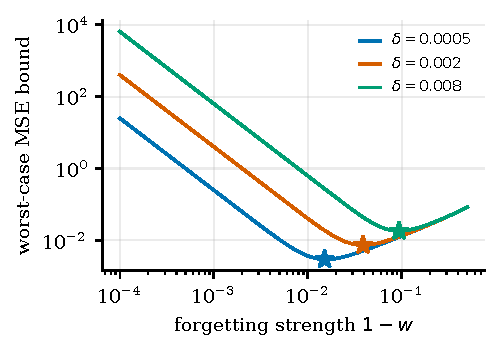
\includegraphics[width=0.93\linewidth]{figs/drift_tradeoff.pdf}
\caption{Bias--variance bounds in Proposition~\ref{prop:drift}. Stars
mark the minimizing forgetting strength; as drift $\delta$ increases,
the optimum moves at the rate in Corollary~\ref{cor:rate}.}
\label{fig:tradeoff}
\end{figure}

\subsection{Finite candidate selection}

\begin{proposition}[Conditional finite-class bound]
\label{prop:oracle}
Let $R(c)$ be the expected validation risk of candidate $c$ and
$\hat R(c)$ its average over $n$ validation items. If the item losses are
independent conditional on the fitted candidates and lie in $[0,B]$, then
the minimizer $\hat c$ over $M$ candidates satisfies, with probability at
least $1-\eta$,
\[
R(\hat c)\le\min_cR(c)+B\sqrt{\frac{2\log(2M/\eta)}{n}}.
\]
\end{proposition}

The independent units are items, because observations and quantiles are
averaged within item before selection. The released selector does not
clip scaled pinball loss, so the bounded-loss assumption is not automatic
and this proposition is not presented as a formal guarantee for the
unclipped implementation. It records the standard finite-class behavior
under an explicit clipping condition.

\subsection{Classical credibility}

\begin{proposition}[Pooling reduces Bayes risk in the stationary model]
\label{prop:credibility}
Under the undiscounted Beta--Binomial occurrence model with known
hyperparameters, the posterior mean is the Bayes estimator of $\pi_i$
under squared loss and has strictly smaller Bayes risk than the per-item
empirical rate whenever $\phi_g>0$. Its optimal weight is the classical
credibility factor $\lambda_i=n_i/(n_i+\phi_g)$
\citep{buhlmann1967}.
\end{proposition}

This is the B\"uhlmann--Straub result specialized to Bernoulli
occurrences. It justifies pooling when the stationary hierarchical model
is correctly specified; it does not assert that a misspecified or stale
group prior helps under drift.

\section{Proofs}\label{app:proofs}

\subsection{Proof of Proposition~\ref{prop:tsb-limit}}
(i) Immediate from \eqref{eq:disc-post} since $c(w),n(w)$ are finite.
(ii) Induction: $\hat p_1=(1-w)p_1+w\hat p_0$. If the closed form holds at
$T-1$, then
$\hat p_T=(1-w)p_T+w\hat p_{T-1}=(1-w)\sum_{t=1}^{T}w^{T-t}p_t+w^{T}\hat p_0$.
With $n(w)=(1-w^{T})/(1-w)$,
\[
\bar p(w)=\frac{(1-w)\sum_t w^{T-t}p_t}{1-w^{T}}
=\frac{\hat p_T-w^{T}\hat p_0}{1-w^{T}}.
\]
(iii) Rearranging, $\bar p(w)-\hat p_T=w^{T}(\bar p(w)-\hat p_0)$, and
$|\bar p(w)-\hat p_0|\le1$. \qed

\subsection{Proof of Proposition~\ref{prop:active}}
$n(w)=(1-w^{T})/(1-w)\le1/(1-w)$ and $x\mapsto x/(x+\phi)$ is increasing,
so $\lambda(w)\le[1/(1-w)]/[1/(1-w)+\phi]=1/(1+(1-w)\phi)$. \qed

\subsection{Proof of Proposition~\ref{prop:drift} and
Corollary~\ref{cor:rate}}
With $k=T-t$ and $\sum_{k\ge0}kw^k=w/(1-w)^2$,
\[
\bigl|\E\bar p(w)-\pi_T\bigr|
=\Bigl|\frac{\sum_t w^{T-t}(\pi_t-\pi_T)}{n(w)}\Bigr|
\le\frac{\delta\,w/(1-w)^2}{(1-w^{T})/(1-w)}
=\delta\,\frac{w}{(1-w)(1-w^{T})}.
\]
By independence and $\pi_t(1-\pi_t)\le\tfrac14$,
\[
\Var\,\bar p(w)\le\frac{\tfrac14\,(1-w^{2T})/(1-w^{2})}
{[(1-w^{T})/(1-w)]^{2}}
=\frac14\cdot\frac{(1-w)(1+w^{T})}{(1+w)(1-w^{T})}.
\]
Decomposing
$\hat\pi-\pi_T=\lambda(\bar p-\E\bar p)+\lambda(\E\bar p-\pi_T)+(1-\lambda)(\mu_\pi-\pi_T)$,
the first term is zero-mean and independent of the deterministic
remainder, giving
$\E(\hat\pi-\pi_T)^2\le[\lambda\mathrm{B}(w)+(1-\lambda)|\mu_\pi-\pi_T|]^2
+\lambda^2\Var\bar p(w)$ with $\mathrm{B}(w)$ the bias bound. For the
corollary set $b=1-w$ and let $T\to\infty$ (so $w^{T}\to0$): the squared
bias bound behaves as $\delta^2(1-b)^2/b^2\sim\delta^2/b^2$ and the
variance bound becomes $\tfrac14\, b/(2-b)$, which is $b/8$ to leading
order as $b\to0$. Minimizing $f(b)=\delta^2/b^2+b/8$ gives
$f'(b)=-2\delta^2/b^3+1/8=0$, i.e.,
$b^{*}=(16\delta^{2})^{1/3}=2^{4/3}\delta^{2/3}$, and
$f(b^{*})=O(\delta^{2/3})$. \qed

\subsection{Proof of Proposition~\ref{prop:oracle}}
For each candidate $c$, Hoeffding's inequality for independent scores in
$[0,B]$ gives
$\Pr\bigl(|\hat R(c)-R(c)|>t\bigr)\le2\exp(-2nt^2/B^2)$. A union bound
over the $M$ candidates makes
$\sup_c|\hat R(c)-R(c)|\le t$ hold with probability at least
$1-2M\exp(-2nt^2/B^2)$. Setting the right side to $\eta$ yields
$t=B\sqrt{\log(2M/\eta)/(2n)}$. On this event,
$R(\hat c)\le\hat R(\hat c)+t\le\hat R(c^{*})+t\le R(c^{*})+2t$ with
$c^{*}=\arg\min_c R(c)$, which is the claim with constant
$2t=B\sqrt{2\log(2M/\eta)/n}$. \qed

\subsection{Proof of Proposition~\ref{prop:credibility}}
With known $(\alpha_g,\beta_g)$ and $s_i\mid\pi_i\sim
\mathrm{Bin}(n_i,\pi_i)$, $\pi_i\sim\mathrm{Beta}(\alpha_g,\beta_g)$,
the posterior mean $\hat\pi_i=\lambda_i\bar p_i+(1-\lambda_i)\mu_\pi$
with $\lambda_i=n_i/(n_i+\phi_g)$ minimizes Bayes risk under squared
loss among all estimators (tower property). Restricting to linear
combinations $a\bar p_i+b$, the Bayes risk is
$a^2\,\E[\Var(\bar p_i\mid\pi_i)] + (1-a)^2\Var(\pi_i)$ at the optimal
intercept, minimized at
$a^{*}=\Var(\pi_i)/\bigl(\Var(\pi_i)+\E[\Var(\bar p_i\mid\pi_i)]\bigr)
=\lambda_i$, the B\"uhlmann credibility weight. The minimum is strictly
below the risk of $a=1$ (the empirical rate) whenever
$\Var(\pi_i)<\infty$ and $\phi_g>0$. \qed

\subsection{Proof of Proposition~\ref{prop:twosided} and
Corollary~\ref{cor:resolution}}

\textbf{(i)} $\lambda_i=n_i/(n_i+\kappa_g)$ is increasing in $n_i$, and
$n_i\le\sum_{k\ge0}w^{k}=(1-w)^{-1}$ for $w<1$. Substituting the bound,
$\lambda_i\le\frac{(1-w)^{-1}}{(1-w)^{-1}+\kappa_g}
=\bigl[1+(1-w)\kappa_g\bigr]^{-1}$, which is $<1$ whenever $w<1$ and
$\kappa_g>0$.

\textbf{(ii)} Write $\bar y_i=\mu_i+e_i$ with
$\mu_i\sim N(\mu_g,\tau_g^2)$ and $e_i\sim N(0,s_i)$ independent,
$s_i=\sigma_g^2/n_i$, so $\Var(\bar y_i)=\tau_g^2+s_i$. For the sample
variance $S_g^2=(m_g-1)^{-1}\sum_{i\in g}(\bar y_i-\bar{\bar y})^2$,
independence gives
$\Var(\bar{\bar y})=m_g^{-2}\sum_i(\tau_g^2+s_i)$ and hence
\[
\E[S_g^2]=\frac{\sum_i(\tau_g^2+s_i)-m_g\Var(\bar{\bar y})}{m_g-1}
=\frac{(1-m_g^{-1})\sum_i(\tau_g^2+s_i)}{m_g-1}
=\tau_g^2+\bar s_g ,
\]
exactly, with no balance assumption. The estimator truncates precisely
when $S_g^2\le\bar s_g$. Under the working model $S_g^2$ is
approximately $(\tau_g^2+\bar s_g)\chi^2_{m_g-1}/(m_g-1)$, so
$\Var(S_g^2)\simeq\frac{2}{m_g-1}(\tau_g^2+\bar s_g)^2$ and the
standardized distance from the truncation boundary is
\[
\frac{\E[S_g^2]-\bar s_g}{\sqrt{\Var(S_g^2)}}
=\frac{\tau_g^2}{\sqrt{2/(m_g-1)}\,(\tau_g^2+\bar s_g)}
=\sqrt{\tfrac{m_g-1}{2}}\;\rho_g ,
\]
giving the stated normal approximation for
$\Pr[S_g^2\le\bar s_g]$. The discount bound follows from
$n_i\le(1-w)^{-1}$: $s_i=\sigma_g^2/n_i\ge(1-w)\sigma_g^2$ for every
$i$, hence $\bar s_g\ge(1-w)\sigma_g^2$, and $\rho_g$ is decreasing in
$\bar s_g$. Finally $\hat\tau_g^2=0$ gives $\kappa_g=\infty$ and
$\lambda_i=0$.

\textbf{Corollary.} Requiring the collapse probability to stay below a
fixed level is, by (ii), the condition $\rho_g\sqrt{(m_g-1)/2}\ge c$ for
a constant $c$ of order one. Solving
$\rho_g=\tau_g^2/(\tau_g^2+\bar s_g)\ge c\sqrt{2/(m_g-1)}$ for
$\tau_g^2$ gives
$\tau_g^2\ge\bar s_g\,c\sqrt{2}/(\sqrt{m_g-1}-c\sqrt2)$, i.e.\ the
stated order $\bar s_g/(\sqrt{m_g-1}-1)$ up to the constant. Refining a
partition decreases $m_g$ and, by construction of the mixture objective,
$\tau_g^2$, while decreasing $w$ raises the floor $(1-w)\sigma_g^2$ on
$\bar s_g$. Each shrinks the left side or raises the right side. \qed

The algebraic steps, the exact unbiasedness in (ii), and the monotonicity
claims are verified with a computer algebra system in
the released test suite. The $\chi^2$ approximation in (ii) is checked
against Monte Carlo simulation, agreeing to within $0.05$ in probability
across the regimes we use.

\section{Implementation details}\label{app:implementation}

\paragraph{EB fitting.} Group Beta--Binomial hyperparameters maximize the
(weighted) marginal likelihood by L-BFGS-B with positivity bounds; the
size block uses pooled within-item variance for $\sigma^2_g$ and an
intercept-only restricted marginal likelihood in $\tau^2_g$ with profiled
$\mu_{0,g}$; item-level process variances use the conjugate
scaled-inv-$\chi^2$ update with $\nu{=}20$. With discounting, every count
is replaced by its weighted analogue \eqref{eq:discounted-stats}; the
Beta--Binomial marginal extends to real pseudo-counts via log-Gamma
functions. The predictive law is zero-inflated log-normal with predictive
variance $\hat\sigma^2_{\mathrm{proc}}+\hat v_\mu$. The released
configuration averages quantiles over $B{=}20$ bootstrap resamples of the
item-statistics rows. An optional location-scale calibration layer exists
but is \emph{off} in all headline results; the adaptive conformal
comparison is reported as a separate baseline rather than used to modify
\REMIX{} after fitting.

\paragraph{Mixture EM.} Deterministic quantile initialization over
(occurrence rate, mean log-size); degenerate components (mass $<2$)
frozen to global fallback priors; tolerance $10^{-5}$, max 60 iterations;
$K\in\{1,\dots,6\}$ by BIC with $5K+(K-1)$ parameters.

\paragraph{Selection.} Internal chronological split (first 80\% / last
20\%, min head 8); score = mean pinball over $q\in\{0.5,0.75,0.9\}$,
per-series scaled by head mean absolute demand, averaged within item and then
uniformly across items; grid over
$w\in\{1,0.999,0.997,0.995,0.99,0.98,0.95,0.90\}$ and partitions
\{global, taxonomy, mixture(BIC)\}. Selected configurations per dataset
are reported beneath Table~\ref{tab:point}; diagnostics
(\texttt{remix\_selection\_diagnostics.csv}) accompany every run.

\paragraph{Environment and timing methodology.} All experiments ran on one
Windows~11 workstation (Intel Core Ultra~9 275HX, 32\,GB RAM). Core
determinism tests are bit-identical within this environment;
cross-environment bit identity is not claimed. Timing is wall-clock and
excludes data loading. Joint selection over the 24 candidates takes
$51$--$243$ seconds per panel, with one deterministic six-$K$ EM/BIC
search for the mixture on the fitting head. Final model-only point plus
five-quantile prediction with $B=20$ takes 6.2 seconds on
Carparts, 38.0 on Online Retail, and 124.0 on M5, whose
external span has 3.235 million observations. GPU is not used in \REMIX{}.

\paragraph{Baselines.} StatsForecast defaults; TSB
$(\alpha_d,\alpha_p)=(0.5,0.45)$; AutoARIMA/AutoTheta season 7 (daily) /
12 (monthly) for intervals. TSB-tuned: $5\times5$ grid
$\alpha_d\in\{0.05,0.1,0.2,0.35,0.5\}$,
$\alpha_p\in\{0.01,0.05,0.1,0.25,0.45\}$ (25 candidates, the same order
as \REMIX{}'s 24), scored on the identical 80/20 chronological split by
per-series scaled MAE (so neither method is scored on its home
criterion), refit on the full window. Selected $(\alpha_d,\alpha_p)$:
Online Retail $(0.10,0.25)$; M5 $(0.20,0.01)$; Auto $(0.20,0.10)$;
Carparts $(0.50,0.45)$, i.e.\ the textbook constants; RAF
$(0.50,0.25)$. Static conformal wrappers use a chronological 80/20 split
and a \emph{panel-pooled} signed-residual distribution; quantiles are
zero-truncated and monotonized. The ACI variants retain that residual
pool and adapt the requested level for every series--quantile pair with
$\gamma=0.05$. Tweedie-GLM is a per-series autoregressive GLM with log
link, $p{=}1.5$, 14 lags (daily) / 6 (monthly), and $\ell_2{=}0.1$.
TweedieGP uses the authors' official implementation with Tweedie
likelihood, median-demand scaling, RBF kernel, and 50{,}000 predictive
samples; zero-only training series receive a zero fallback so that every
series is scored. iETS uses \texttt{smooth::adam} with automatic
occurrence modeling.

\section{Additional results}\label{app:extra}

% -------------------------------------------------------------------------
\subsection{Point forecasting and horizon decomposition}
\label{app:point}

Table~\ref{tab:point} gives the complete point comparison retained for
continuity with the intermittent-demand literature. Rankings exclude the
deliberately degenerate Zero and Naive-last rows. \REMIX{} takes six of
ten MAE/RMSSE cells and is top two on seven, but the result is not uniform:
classical methods retain several point-metric wins, and Zero attains the
lowest MAE on Online Retail, Carparts, and RAF. This is why the main text
uses point accuracy as a secondary diagnostic.

\begin{table*}[t]
\centering
\caption{Point forecasting across the five panels (lower is better;
bold best and underline second among non-degenerate methods). Degenerate
rows are shown as metric diagnostics and excluded from ranking.}
\label{tab:point}
\small
\setlength{\tabcolsep}{3.4pt}
\begin{tabular}{lcc@{\hspace{10pt}}cc@{\hspace{10pt}}cc@{\hspace{10pt}}cc@{\hspace{10pt}}cc}
\toprule
 & \multicolumn{2}{c}{Online Retail} & \multicolumn{2}{c}{M5} & \multicolumn{2}{c}{Auto} & \multicolumn{2}{c}{Carparts} & \multicolumn{2}{c}{RAF}\\
\cmidrule(lr){2-3}\cmidrule(lr){4-5}\cmidrule(lr){6-7}\cmidrule(lr){8-9}\cmidrule(lr){10-11}
Model & MAE & RMSSE & MAE & RMSSE & MAE & RMSSE & MAE & RMSSE & MAE & RMSSE\\
\midrule
CrostonClassic & 6.3294 & 5.1051 & 1.2345 & 2.3539 & 3.4056 & 1.1488 & 0.6792 & 1.0981 & 2.7315 & 1.6280\\
CrostonSBA & 6.1953 & 5.0692 & 1.2076 & 2.3517 & \secondbest{3.3325} & \secondbest{1.1451} & 0.6628 & 1.0935 & 2.6520 & 1.6272\\
TSB & \secondbest{5.5736} & 4.8031 & 1.2672 & 2.3612 & 3.6587 & 1.2066 & \best{0.5396} & 1.0156 & \best{2.1660} & 1.6570\\
TSB-tuned & 5.6318 & 4.7985 & \best{1.1932} & \secondbest{2.3137} & 3.3917 & 1.1452 & \best{0.5396} & 1.0156 & \secondbest{2.2447} & 1.6408\\
ADIDA & 5.6860 & \secondbest{4.7967} & 1.2274 & 2.3398 & 3.4079 & 1.1545 & 0.5556 & 1.0244 & 2.2977 & \secondbest{1.6245}\\
IMAPA & 5.7000 & 4.7970 & 1.2317 & 2.3280 & 3.4143 & 1.1555 & \secondbest{0.5524} & 1.0126 & 2.2850 & 1.6259\\
AutoARIMA & 6.5494 & 4.8175 & 1.2283 & 2.3169 & 3.4417 & 1.1745 & 0.5822 & \secondbest{1.0105} & 2.3153 & 1.6262\\
AutoTheta & 8.2862 & 4.8550 & 1.2988 & 2.3143 & 3.7490 & 1.2215 & 0.5704 & \best{0.9966} & 2.3687 & 1.6399\\
\midrule
Zero & 4.7549 & 4.8089 & 1.2995 & 2.4629 & 4.1444 & 1.4454 & 0.3867 & 1.0949 & 1.1717 & 1.6345\\
Naive-last & 6.0570 & 4.8324 & 1.3750 & 2.5450 & 4.3529 & 1.3818 & 0.5399 & 1.1408 & 1.8340 & 1.7644\\
\midrule
\REMIX{} (ours) & \best{5.5325} & \best{4.7901} & \secondbest{1.2032} & \best{2.2938} & \best{3.2145} & \best{1.1374} & 0.5726 & 1.0120 & 2.3874 & \best{1.6245}\\
\bottomrule
\end{tabular}
\end{table*}

\begin{figure}[t]
\centering
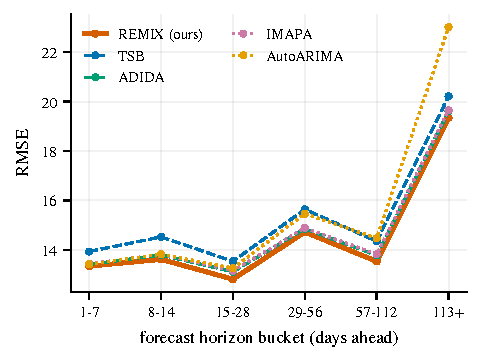
\includegraphics[width=0.93\linewidth]{figs/horizon_decomp.pdf}
\caption{Online Retail RMSE by fixed-origin forecast-horizon bucket.
\REMIX{} is lowest in every bucket, so the aggregate result is not
created by averaging only over distant horizons. MAE differences among
the leading methods are within $1$--$2\%$ by bucket.}
\label{fig:horizon}
\end{figure}

The selected $(g,w)$ pairs are: Online Retail (global, $0.95$), M5
(mixture, $0.95$), Auto (global, $0.99$), Carparts (global, $0.90$), and
RAF (mixture, $0.997$). On three of the five panels the margins between
pooling structures on the internal validation surface are under a tenth
of a percent, so the structure component of these pairs should be read as
Section~\ref{sec:leverage} reads it: the selector avoids poor structural
corners, and no winner is announced where the surface does not resolve
one.

\subsection{Selector diagnostics}
\label{sec:selector-diagnostics}
\label{app:selector-diagnostics}

The selection surface is locally flat near its optimum: on Online Retail
the best seven candidates span all three pooling structures and lie within
$0.51\%$ of one another in validation SPL. Section~\ref{sec:leverage}
reports the credibility leverage and refinement gains that accompany each
selected pair, and Figure~\ref{fig:refinement-leverage} places them
against the controlled panels. The selector is useful for choosing a
discount and for avoiding poor structural corners; the winning pooling
structure on a panel whose candidates lie within a tenth of a percent
should not be read as a scientific taxonomy. Per-panel selection surfaces
are released with the code.

\begin{table*}[t]
\centering
\caption{Full Online Retail ablation corresponding to
Table~\ref{tab:ablation}. Each row is an independent run; ``auto'' denotes
its own internal discount selection. TSB has no native predictive
distribution. Lower is better.}
\label{tab:ablation-full}
\small
\setlength{\tabcolsep}{5.0pt}
\begin{tabular}{llrrrrrr}
\toprule
Pooling & Forget & MAE & RMSE & RMSSE & SPL & SPL$_{90}$ & AIW\\
\midrule
none (TSB) & fixed & 5.5736 & 18.7272 & 4.8031 & --- & --- & ---\\
global & off & 5.7623 & \best{17.6892} & \best{4.7851} & 0.8899 & 1.5306 & 10.51\\
taxonomy & off & 5.7663 & \secondbest{17.6930} & \secondbest{4.7875} & 0.8897 & 1.5299 & 10.56\\
learned & off & 5.8126 & 17.7064 & 4.7876 & 0.8905 & 1.5336 & 10.79\\
global & auto ($.95$) & \best{5.5325} & 17.8386 & 4.7901 & \secondbest{0.8849} & \secondbest{1.5268} & \best{9.25}\\
taxonomy & auto ($.95$) & \secondbest{5.5624} & 17.8421 & 4.7897 & \best{0.8846} & \best{1.5254} & 9.43\\
learned & auto ($.95$) & 5.6925 & 17.8765 & 4.7902 & 0.8869 & 1.5343 & 10.69\\
\bottomrule
\end{tabular}
\end{table*}

\subsection{Walk-forward point results and protocol}
\label{app:walkforward}

\begin{table}[t]
\centering
\caption{Online Retail point forecasting under strict seven-day
walk-forward updates. The hierarchical rows differ in their
initialization discount and pooling structure.}
\label{tab:walkforward}
\small
\setlength{\tabcolsep}{5pt}
\begin{tabular}{lccc}
\toprule
Model & MAE & RMSE & RMSSE\\
\midrule
CrostonClassic & 5.692 & 16.937 & 4.854\\
CrostonSBA & 5.586 & 16.931 & 4.836\\
TSB & 5.434 & 17.754 & 4.815\\
ADIDA & \best{5.320} & \best{16.728} & \secondbest{4.637}\\
IMAPA & \secondbest{5.332} & \secondbest{16.745} & \best{4.632}\\
AutoARIMA & 5.482 & 16.904 & 5.105\\
AutoTheta & 5.394 & 16.836 & 4.735\\
\midrule
Stationary hierarchy ($w=1$) & 5.586 & 17.260 & 4.725\\
Forgetting hierarchy (tax., $.95$) & 5.411 & 17.059 & 4.682\\
\REMIX{} (selected global, $.95$) & 5.421 & 17.188 & 4.696\\
\bottomrule
\end{tabular}
\end{table}

\begin{table*}[t]
\centering
\caption{Full Online Retail probabilistic walk-forward results. SPL is
reported at all five quantiles and on average; Cov@80 is marginal
coverage and Cov$^{+}$@80 conditions on positive demand. CP and ACI
wrappers refit each block; AutoARIMA, AutoTheta, and iETS refit every four
blocks; \REMIX{} updates sufficient statistics each block.}
\label{tab:wfprob-full}
\small
\setlength{\tabcolsep}{4.2pt}
\begin{tabular}{lrrrrrrrr}
\toprule
Model & q10 & q25 & q50 & q75 & q90 & Mean & Cov@80 & Cov$^{+}$@80\\
\midrule
CP-Croston & 0.341 & 0.778 & 1.364 & 1.745 & 2.632 & 1.372 & 0.793 & 0.479\\
CP-SBA & 0.334 & 0.762 & 1.343 & 1.725 & 2.722 & 1.377 & 0.793 & 0.482\\
CP-TSB & 0.451 & 0.899 & 1.289 & 1.385 & 2.842 & 1.373 & 0.795 & 0.468\\
CP-ADIDA & 0.277 & 0.627 & 1.050 & \secondbest{1.319} & 2.514 & 1.158 & 0.791 & 0.473\\
CP-IMAPA & 0.292 & 0.660 & 1.084 & 1.329 & 2.522 & 1.177 & 0.791 & 0.471\\
AutoARIMA & 0.259 & 0.572 & 1.197 & 1.763 & 1.522 & 1.063 & 0.933 & 0.762\\
AutoTheta & 0.232 & 0.584 & 1.276 & 1.717 & \secondbest{1.483} & 1.059 & 0.931 & 0.765\\
iETS & 0.236 & 0.505 & 1.302 & 1.562 & 1.940 & 1.109 & 0.598 & 0.166\\
ACI-ADIDA & \secondbest{0.186} & \secondbest{0.468} & \best{0.909} & 1.324 & 1.668 & \secondbest{0.911} & 0.904 & 0.646\\
ACI-TSB & 0.189 & 0.482 & 0.948 & 1.384 & 1.709 & 0.942 & 0.904 & 0.641\\
Zero (diagnostic) & 0.183 & 0.458 & 0.916 & 1.374 & 1.649 & 0.916 & 0.740 & 0.000\\
\midrule
\REMIX{} & \best{0.183} & \best{0.458} & \secondbest{0.910} & \best{1.319} & \best{1.400} & \best{0.854} & 0.901 & 0.621\\
\bottomrule
\end{tabular}
\end{table*}

\begin{table*}[t]
\centering
\caption{Full Carparts monthly walk-forward SPL. Every statistical
baseline refits each block; \REMIX{} updates sufficient statistics.
The zero row is excluded from ranking.}
\label{tab:wf-carparts-full}
\small
\setlength{\tabcolsep}{5pt}
\begin{tabular}{lrrrrrr}
\toprule
Model & q10 & q25 & q50 & q75 & q90 & Mean\\
\midrule
AutoARIMA & 0.151 & 0.282 & 0.537 & 0.644 & 0.484 & 0.419\\
AutoTheta & 0.120 & 0.253 & 0.523 & 0.658 & \secondbest{0.474} & 0.406\\
CP-TSB & 0.141 & 0.301 & 0.487 & \secondbest{0.513} & 0.476 & 0.384\\
CP-ADIDA & \secondbest{0.096} & \secondbest{0.230} & \secondbest{0.411} & 0.529 & 0.488 & 0.351\\
CP-IMAPA & 0.101 & 0.235 & 0.413 & 0.518 & 0.479 & \secondbest{0.349}\\
iETS & 0.272 & 0.368 & 0.493 & 0.532 & 0.515 & 0.436\\
Zero (diagnostic) & 0.075 & 0.187 & 0.374 & 0.560 & 0.672 & 0.374\\
\midrule
\REMIX{} & \best{0.075} & \best{0.187} & \best{0.372} & \best{0.481} & \best{0.458} & \best{0.315}\\
\bottomrule
\end{tabular}
\end{table*}

\REMIX{} applies the selected discount once to the initialization
sufficient statistics and then accumulates revealed blocks without
compounding it. On Online Retail, ACI-ADIDA improves the static conformal
wrapper substantially and wins q50 by a hair, but \REMIX{} takes every
other quantile, the mean, and q90 by a clear margin. On Carparts the
first two quantiles saturate at zero and the discriminating gains occur
from the median up. Re-running joint selection at every block is not
evaluated.

\subsection{Significance and interval diagnostics}
\label{sec:significance}

\begin{table}[t]
\centering
\caption{Per-series mean SPL paired tests: \REMIX{} versus every
comparator on each panel, Holm-adjusted within panel (paired $t$ and
Wilcoxon signed-rank; the family includes TweedieGP on the monthly
panels). Cells count comparators by outcome at the $5\%$ level; named
entries are the comparators for which \REMIX{} is \emph{not}
significantly better.}
\label{tab:spl-significance}
\small
\setlength{\tabcolsep}{4.0pt}
\begin{tabular}{lcccl}
\toprule
Panel & Family & Sig.\ better & Sig.\ worse & Undecided\\
\midrule
Online Retail & 9 & 9 & 0 & ---\\
M5 & 9 & 5 & 0 & CP wrappers (4)\\
Auto & 10 & 10 & 0 & ---\\
Carparts & 10 & 9 & 0 & TweedieGP\\
RAF & 10 & 10 & 0 & ---\\
\bottomrule
\end{tabular}
\end{table}

\begin{table}[t]
\centering
\caption{Paired per-series MAE tests on Online Retail: \REMIX{} versus
each alternative. Negative mean differences favor \REMIX{}; $p$-values
are Holm-adjusted.}
\label{tab:significance}
\small
\setlength{\tabcolsep}{5pt}
\begin{tabular}{lccc}
\toprule
vs. & Mean diff & $p_t$ & $p_{\mathrm{Wilcoxon}}$\\
\midrule
Stationary hierarchy & $-0.165$ & $<10^{-29}$ & $<10^{-11}$\\
TSB & $-0.040$ & $0.532$ & $<10^{-155}$\\
TSB-tuned & $-0.090$ & $0.086$ & $<10^{-72}$\\
ADIDA & $-0.036$ & $0.359$ & $<10^{-88}$\\
IMAPA & $-0.049$ & $0.281$ & $<10^{-97}$\\
CrostonSBA & $-0.872$ & $<10^{-26}$ & $<10^{-59}$\\
AutoARIMA & $-0.891$ & $<10^{-14}$ & $<10^{-12}$\\
AutoTheta & $-2.644$ & $<10^{-81}$ & $<10^{-104}$\\
\bottomrule
\end{tabular}
\end{table}

\begin{table}[t]
\centering
\caption{Raw \REMIX{} interval quality across panels at nominal $80\%$
coverage. No post-hoc calibration is used.}
\label{tab:coverage}
\small
\setlength{\tabcolsep}{4.6pt}
\begin{tabular}{lccccc}
\toprule
 & OR & M5 & Auto & Carparts & RAF\\
\midrule
Coverage@80 & 0.892 & 0.846 & 0.907 & 0.931 & 0.921\\
AIW@80 & 9.25 & 2.81 & 9.21 & 1.47 & 0.94\\
\bottomrule
\end{tabular}
\end{table}

Table~\ref{tab:spl-significance} tests the headline metric directly:
per-series mean SPL, \REMIX{} against every comparator of
Table~\ref{tab:prob}, with paired $t$ and Wilcoxon signed-rank tests
Holm-adjusted within each panel and a comparison counted as decided only
when both adjusted tests agree at the $5\%$ level. \REMIX{} is
significantly better in 43 of the 48 panel--comparator pairs and
significantly worse in none. The five undecided pairs are informative
rather than embarrassing: on M5 the mean difference favors \REMIX{}
against all four conformal wrappers but the paired $t$ does not reach
significance after correction (the Wilcoxon strongly rejects symmetry,
so the per-series differences are systematic but heavy-tailed), and on
Carparts neither \REMIX{} nor TweedieGP separates from the other
(adjusted $p\ge0.50$ both ways), consistent with the half-percent
aggregate margin between them.

The paired MAE tests support a systematic improvement over the stationary
hierarchy. Against TSB, tuned TSB, ADIDA, and IMAPA, mean MAE favors
\REMIX{} but the adjusted paired $t$-tests are not significant; the
Wilcoxon tests reverse because those methods win on the typical series
while \REMIX{} reduces the difficult-series tail. On per-series RMSE,
both adjusted tests favor \REMIX{} against every comparator at $p<0.05$.
Raw intervals mildly over-cover, most strongly on Carparts.

\begin{figure}[t]
\centering
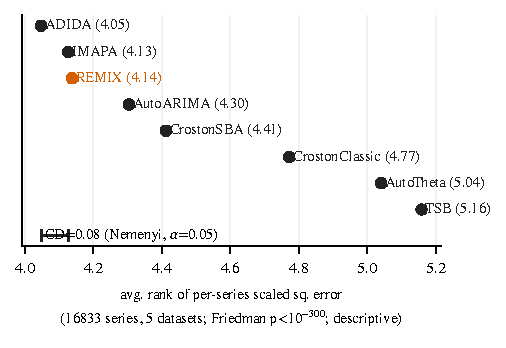
\includegraphics[width=0.93\linewidth]{figs/cd_diagram.pdf}
\caption{Average ranks of per-series scaled squared errors over the
16{,}833 series with complete saved row-level point predictions across
the five panels. The critical-difference bar is shown only for scale:
series, rather than datasets, are the blocks, so this is descriptive and
not a valid Friedman--Nemenyi test.}
\label{fig:cd}
\end{figure}

\subsection{Selection objective and efficiency}
\label{sec:criterion}\label{sec:efficiency}

The selector is not mathematically tied to pinball loss; it scores the
criterion supplied on the chronological validation tail. We use
item-averaged SPL because the target is a predictive distribution. The
best candidates are locally close, and a full cross-objective regret
matrix remains future work.

Joint selection takes $51$--$243$ seconds across the five panels,
excluding data loading, and covers 24 forecast candidates with one
deterministic EM/BIC search for the mixture on the fitting head. Final
estimation is analytic apart from low-dimensional group optimization;
selection and point prediction are deterministic, while probabilistic
bootstrap averaging uses the released fixed seed.

\subsection{Controlled-study diagnostics}
\label{app:simulation-details}

In the length sweep used to isolate credibility leverage, the generator
holds $K=2$, 500 items per group, occurrence probabilities $0.05$ and
$0.80$, log-size centers three units apart, and $w=1$. The true
partition's pinball advantage falls monotonically from $1.53\%$ at
$T=12$ (median 4.5 positives per item) to $0.01\%$ at $T=400$ (median
154), with NLL, Brier, and log-size MSE following the same direction.
Across the main grid, the RMSE of $\hat\tau_g^2$ approximately doubles
as $w$ falls from $1.00$ to $0.90$ ($0.037\to0.144$ at $T=120$ and
$0.074\to0.149$ at $T=30$), directly measuring the resolution cost in
Proposition~\ref{prop:twosided}.

The generator centers the groups symmetrically around a fixed grand mean
so that increasing separation does not change total demand scale, and
every arm is evaluated through the same hurdle-lognormal predictive
representation under both likelihood-based proper scores and point
metrics. A four-arm ladder---single pool, true labels with estimated
hyperparameters, true labels with true hyperparameters, and the true
conditional law---checks the implementation; the true conditional law is
best on every metric in every cell.


\subsection{Released tables and artifacts}
Complete per-dataset tables with RMSE, WRMSSE, all quantile levels,
coverage, interval widths, fixed-corner ablations, and runtimes accompany
the code release, together with the selection surfaces and per-run
diagnostics behind every table in this paper.

\subsection{Machine-readable significance output}
The complete per-series results behind Table~\ref{tab:significance} and
Table~\ref{tab:spl-significance}, including the RMSE tests and the
Holm-adjusted families, accompany the code release as machine-readable
CSV files.

\subsection{MASE}
For completeness we report MASE (per-series MAE scaled by in-sample
naive MAE), the intermittent-demand literature's traditional point
metric. It inherits the absolute-error pathology quantified in
Section~\ref{sec:main-results}: the all-zero forecast attains the best
MASE on Online Retail ($1.84$ vs.\ TSB $2.08$, \REMIX{} $2.41$),
Carparts, and RAF, and zero-leaning methods (TSB, IMAPA) lead among real
forecasters. On Auto, \REMIX{} ($0.889$) is second only to CrostonSBA
($0.883$). Full table in the repository
(\texttt{mase\_table.csv}). We treat MASE as descriptive, not
decision-relevant, for the same reason as MAE.

\subsection{Walk-forward artifacts}
The complete point and probabilistic results are in
Tables~\ref{tab:walkforward} and \ref{tab:wfprob}; released block-level
artifacts retain the seven-day boundaries and every per-block prediction.

\subsection{Neural baselines}
\label{app:neural}

Table~\ref{tab:neural} retains the earlier neural comparisons. Deep
Renewal Processes (DRP) \citep{turkmen2019} are architecturally close to
our occurrence--size decomposition, but the legacy subsample numbers are
indicative only: we rebuilt the Python~3.8/MXNet~1.7 environment and
launched the original code path, yet three configurations diverged to
NaN between epochs 7 and 11 and failed during prediction. DeepAR and an
RNN under prediction-only chaining reach lower MAE in one case but worse
RMSE and RMSSE at both horizons. Neural decoding and a constant
sufficient-statistic forecast are not timing-equivalent, so these rows
should not support a broad efficiency ratio.

Two newly executed reference points provide a cleaner, narrower check.
DeepState---the published Amazon ISSM successor available in GluonTS,
not a reproduction of \citet{seeger2016}---obtains mean SPL $1.0652$ on
a 1{,}000-series Online Retail subset and $0.4608$ on full Carparts.
Chronos-Bolt-small obtains $0.8448$ on an Online Retail 500-series subset,
versus $0.8342$ for \REMIX{} on exactly the same subset: a small $1.3\%$
gap. Its Carparts result is only a reference point because the same-source
Monash panel appears in the Chronos data repository and potential training
contamination cannot be excluded. These subset results motivate an
efficiency, determinism, and transparency claim, not a large foundation-
model accuracy advantage.

\begin{table}[t]
\centering
\caption{Neural comparisons on Online Retail. Top: probabilistic
(unscaled pinball, 500-series subsample, fixed protocol). Bottom: point
metrics under prediction-only chaining at two horizons.}
\label{tab:neural}
\small
\setlength{\tabcolsep}{4pt}
\begin{tabular}{lcccccc}
\toprule
 & q10 & q25 & q50 & q75 & q90 & Time\\
\midrule
DeepRenewal & 0.358 & 0.895 & 1.790 & 2.684 & 2.941 & $\sim$20\,min\\
Hierarchical EB & 0.387 & 0.914 & 1.772 & 2.390 & 2.186 & 1\,s\\
\midrule
 & \multicolumn{2}{c}{MAE} & \multicolumn{2}{c}{RMSE} & \multicolumn{2}{c}{RMSSE}\\
 & $h{=}10$ & $h{=}100$ & $h{=}10$ & $h{=}100$ & $h{=}10$ & $h{=}100$\\
\midrule
RNN & 3.257 & 3.132 & 11.938 & 12.538 & 0.875 & 8.197\\
DeepAR & 6.245 & 7.288 & 17.221 & 18.623 & 7.151 & 9.986\\
Hierarchical EB & 4.639 & 4.495 & 11.284 & 11.733 & 0.855 & 8.170\\
\bottomrule
\end{tabular}
\end{table}

\subsection{Far-tail quantiles on the sparsest panels}
\label{app:fartail}

Scaled pinball at $q\in\{0.95,0.975,0.99\}$ on the two panels where the
standard levels discriminate weakly, under the identical fixed protocol
(REMIX raw, $B{=}20$; iETS not re-run at these levels). The zero
forecast's scaled pinball is \emph{linear} in $q$ (its pinball at level
$q$ is $q\,\E[y/\mathrm{scale}]$), so the far tail is exactly where its
apparent advantage must collapse; the question the table answers is who
inherits the lead.

\begin{table}[h]
\centering
\small
\setlength{\tabcolsep}{3.6pt}
\begin{tabular}{lccc@{\hspace{10pt}}ccc}
\toprule
 & \multicolumn{3}{c}{Carparts} & \multicolumn{3}{c}{RAF}\\
\cmidrule(lr){2-4}\cmidrule(lr){5-7}
Model & q95 & q97.5 & q99 & q95 & q97.5 & q99\\
\midrule
CP-Croston & 0.413 & 0.290 & 0.168 & 0.488 & 0.537 & 0.526\\
CP-SBA & 0.412 & 0.290 & 0.168 & 0.489 & 0.542 & 0.529\\
CP-TSB & 0.374 & 0.263 & 0.160 & 0.506 & 0.601 & 0.552\\
CP-ADIDA & 0.384 & 0.275 & 0.159 & 0.493 & 0.579 & 0.557\\
CP-IMAPA & 0.378 & 0.270 & 0.156 & 0.493 & 0.581 & 0.564\\
AutoARIMA & 0.385 & 0.332 & 0.301 & \best{0.460} & 0.395 & 0.356\\
AutoTheta & 0.367 & 0.316 & 0.285 & 0.464 & 0.399 & 0.359\\
Tweedie-GLM & 0.581 & 0.445 & 0.305 & 0.497 & 0.439 & 0.367\\
TweedieGP & \best{0.355} & \best{0.222} & \best{0.128} & 0.462 & \best{0.352} & \secondbest{0.247}\\
\midrule
Zero & 0.710 & 0.729 & 0.740 & 0.507 & 0.520 & 0.529\\
\midrule
\REMIX{} & \secondbest{0.365} & \secondbest{0.251} & \secondbest{0.144} & \secondbest{0.461} & \secondbest{0.364} & \best{0.246}\\
\bottomrule
\end{tabular}
\end{table}

Three readings follow. First, \textbf{the saturation breaks as expected}:
on RAF the zero forecast, marginally ahead at $q\le0.9$, falls behind
every intensity-bearing method from $q{=}0.95$ on, and on Carparts it is
last by a factor of two. Second, \textbf{tail leadership is
model-specific}: official TweedieGP wins all three Carparts cells, while
\REMIX{} is second in all three; on RAF, AutoARIMA wins q95, TweedieGP
wins q97.5, and \REMIX{} wins q99 by a near tie. Third, this table
deliberately narrows the claim: \REMIX{}'s most consistent advantage is
aggregate SPL, not universal extreme-quantile dominance. The conformal
wrappers still deteriorate in the RAF far tail, where their per-level
calibration information is sparse.

\subsection{Full-posterior inference on the same hierarchy}
\label{app:mcmc}

To separate the inference method from the model, we paired plug-in EB
with a full-posterior sampler at each discount. Each pair uses the same
single global pool, shared size-variance specification, discounted
sufficient statistics, seed-controlled 500-series Online Retail subsample,
evaluation span, and scoring code. The sampler uses
Metropolis-within-Gibbs for the Beta hyperparameters, four deterministic
chains of 4{,}000 sweeps, 2{,}000 burn-in iterations, and thinning by four.
Both a stationary version ($w{=}1$) and a power-prior discounted version
($w{=}0.98$) are tested. The richer \REMIX{} arm runs its joint
selection separately on this subsample and is
reported only as context, not as an inference-method contrast.

\begin{table}[h]
\centering
\small
\begin{tabular}{lccccc}
\toprule
 & SPL mean & SPL q90 & MAE & RMSSE & sec.\\
\midrule
\REMIX{} (incl.\ selection) & 0.7942 & 1.3682 & 5.6259 & 4.6712 & 86.4\\
EB global, $w{=}1$ & 0.7919 & 1.3588 & 5.5504 & 4.6684 & 0.2\\
Gibbs global, $w{=}1$ & 0.7919 & 1.3590 & 5.5890 & 4.6696 & 2.7\\
EB global, $w{=}0.98$ & 0.7935 & 1.3658 & 5.4774 & 4.6694 & 0.2\\
Gibbs global, $w{=}0.98$ & 0.7937 & 1.3665 & 5.5549 & 4.6734 & 2.7\\
\bottomrule
\end{tabular}
\end{table}

Two readings. First, \emph{the empirical-Bayes approximation is not a
distributional-accuracy bottleneck}: paired full-posterior inference changes
mean SPL by $0.007\%/0.019\%$, q90 SPL by $0.018\%/0.048\%$, and RMSSE by
$0.025\%/0.085\%$ at $w=1/0.98$. MAE is somewhat more sensitive but still
changes only $0.70\%/1.42\%$. Second, forgetting helps MAE under both
inference methods, so that finding is not an artifact of the EB plug-in.
The maximum split-$\widehat R$ across $(\alpha,\beta,\mu_0,\tau^2,\sigma^2)$
is $1.0021$, and the minimum effective sample size is $819$ of 2{,}000
retained draws.
What this experiment does \emph{not} measure: the richer external
state-space samplers
\citep{chapados2014,seeger2016} remain unrun (Limitations, item~6); this
conjugate single-pool Gibbs is far cheaper than those models and is a
control for the inference method, not a stand-in for them. The plug-in
EB path retains bit-reproducibility and requires no convergence
diagnostics, but at this scale raw speed does not separate the two.

\subsection{Datasets}\label{app:datasets}
Online Retail: UCI 352; returns/zero-price removed, 99.5\% quantity cap,
daily aggregation densified with zeros. M5: Kaggle M5-Accuracy;
seed-controlled 5{,}000-series sample. Both M5 protocols use a two-thirds
initialization split; the learned mixture is selected at $w=0.95$ on all
three audited seeds. Auto/RAF: gluon-ts
\texttt{intermittent-datasets} branch. Carparts: Zenodo 4656022, series
without missing values and with at least one zero (2{,}509). Monthly
panels use the last-$h$ holdout of \citet{damato2025}.

\end{document}
